% ============================================================================
% ANNSIM'27 submission draft -- Modeling and Simulation in Cyber Security track
% NOTE: port to the official SCS/ANNSIM'27 LaTeX template before submission
% (single column, 12-page limit incl. references -- check the CFP).  This file
% uses a neutral article layout so it compiles anywhere.
% ============================================================================
\documentclass[10pt]{article}
\usepackage[letterpaper,margin=1in]{geometry}
\usepackage{times}
\usepackage[T1]{fontenc}
\usepackage[utf8]{inputenc}
\usepackage{amsmath,amssymb}
\usepackage{graphicx}
\usepackage{booktabs}
\usepackage{xcolor}
\usepackage[numbers,sort&compress]{natbib}
\usepackage[hidelinks]{hyperref}
\usepackage{enumitem}
\usepackage{tikz}
\usetikzlibrary{arrows.meta,positioning,fit}
\setlist{nosep,leftmargin=*}

\newcommand{\safeacd}{\textsc{SafeACD-Sim}}
\newcommand{\typed}{\textsc{Typed}}
\newcommand{\todo}[1]{\textcolor{red}{[TODO: #1]}}
\IfFileExists{results_macros.tex}{% Auto-generated by scripts/analyze.py -- do not edit by hand.
\newcommand{\resTrainLagR}{-60.5}
\newcommand{\resTrainLagRIqm}{-58.8}
\newcommand{\resTrainLagProd}{8.1}
\newcommand{\resTrainLagTraf}{54.4}
\newcommand{\resTrainLagEvid}{1.01}
\newcommand{\resTrainLagCrit}{0.11}
\newcommand{\resTrainLagSat}{0.34}
\newcommand{\resTrainLagHardFree}{0.492}
\newcommand{\resTrainLagImpact}{1.0}
\newcommand{\resTrainLagDeployR}{-131.8}
\newcommand{\resTrainLagDeployRIqm}{-102.4}
\newcommand{\resTrainLagDeployProd}{8.5}
\newcommand{\resTrainLagDeployTraf}{89.9}
\newcommand{\resTrainLagDeployEvid}{0.02}
\newcommand{\resTrainLagDeployCrit}{0.00}
\newcommand{\resTrainLagDeploySat}{0.49}
\newcommand{\resTrainLagDeployHardFree}{0.981}
\newcommand{\resTrainLagDeployImpact}{4.4}
\newcommand{\resTrainPlaybookR}{-46.0}
\newcommand{\resTrainPlaybookRIqm}{-46.0}
\newcommand{\resTrainPlaybookProd}{7.9}
\newcommand{\resTrainPlaybookTraf}{41.7}
\newcommand{\resTrainPlaybookEvid}{0.00}
\newcommand{\resTrainPlaybookCrit}{0.00}
\newcommand{\resTrainPlaybookSat}{0.65}
\newcommand{\resTrainPlaybookHardFree}{1.000}
\newcommand{\resTrainPlaybookImpact}{1.5}
\newcommand{\resTrainPpoR}{-1.5}
\newcommand{\resTrainPpoRIqm}{-1.4}
\newcommand{\resTrainPpoProd}{494.1}
\newcommand{\resTrainPpoTraf}{1181.0}
\newcommand{\resTrainPpoEvid}{4.30}
\newcommand{\resTrainPpoCrit}{59.82}
\newcommand{\resTrainPpoSat}{0.00}
\newcommand{\resTrainPpoHardFree}{0.002}
\newcommand{\resTrainPpoImpact}{0.0}
\newcommand{\resTrainPpoDeployR}{-101.6}
\newcommand{\resTrainPpoDeployRIqm}{-61.1}
\newcommand{\resTrainPpoDeployProd}{312.6}
\newcommand{\resTrainPpoDeployTraf}{1021.3}
\newcommand{\resTrainPpoDeployEvid}{0.01}
\newcommand{\resTrainPpoDeployCrit}{0.00}
\newcommand{\resTrainPpoDeploySat}{0.00}
\newcommand{\resTrainPpoDeployHardFree}{0.994}
\newcommand{\resTrainPpoDeployImpact}{5.6}
\newcommand{\resTrainRandomR}{-458.0}
\newcommand{\resTrainRandomRIqm}{-458.0}
\newcommand{\resTrainRandomProd}{328.8}
\newcommand{\resTrainRandomTraf}{1019.4}
\newcommand{\resTrainRandomEvid}{5.86}
\newcommand{\resTrainRandomCrit}{39.97}
\newcommand{\resTrainRandomSat}{0.00}
\newcommand{\resTrainRandomHardFree}{0.000}
\newcommand{\resTrainRandomImpact}{24.0}
\newcommand{\resTrainShapedTenthR}{-14.5}
\newcommand{\resTrainShapedTenthRIqm}{-14.5}
\newcommand{\resTrainShapedTenthProd}{9.4}
\newcommand{\resTrainShapedTenthTraf}{118.0}
\newcommand{\resTrainShapedTenthEvid}{6.33}
\newcommand{\resTrainShapedTenthCrit}{0.01}
\newcommand{\resTrainShapedTenthSat}{0.04}
\newcommand{\resTrainShapedTenthHardFree}{0.038}
\newcommand{\resTrainShapedTenthImpact}{0.1}
\newcommand{\resTrainShapedTenthDeployR}{-116.9}
\newcommand{\resTrainShapedTenthDeployRIqm}{-116.9}
\newcommand{\resTrainShapedTenthDeployProd}{41.3}
\newcommand{\resTrainShapedTenthDeployTraf}{377.1}
\newcommand{\resTrainShapedTenthDeployEvid}{0.35}
\newcommand{\resTrainShapedTenthDeployCrit}{0.00}
\newcommand{\resTrainShapedTenthDeploySat}{0.13}
\newcommand{\resTrainShapedTenthDeployHardFree}{0.740}
\newcommand{\resTrainShapedTenthDeployImpact}{6.3}
\newcommand{\resTrainShapedThreeTenthsR}{-27.3}
\newcommand{\resTrainShapedThreeTenthsRIqm}{-27.3}
\newcommand{\resTrainShapedThreeTenthsProd}{6.8}
\newcommand{\resTrainShapedThreeTenthsTraf}{38.0}
\newcommand{\resTrainShapedThreeTenthsEvid}{4.25}
\newcommand{\resTrainShapedThreeTenthsCrit}{0.04}
\newcommand{\resTrainShapedThreeTenthsSat}{0.04}
\newcommand{\resTrainShapedThreeTenthsHardFree}{0.040}
\newcommand{\resTrainShapedThreeTenthsImpact}{0.2}
\newcommand{\resTrainShapedThreeTenthsDeployR}{-271.4}
\newcommand{\resTrainShapedThreeTenthsDeployRIqm}{-271.4}
\newcommand{\resTrainShapedThreeTenthsDeployProd}{50.7}
\newcommand{\resTrainShapedThreeTenthsDeployTraf}{299.3}
\newcommand{\resTrainShapedThreeTenthsDeployEvid}{0.13}
\newcommand{\resTrainShapedThreeTenthsDeployCrit}{0.00}
\newcommand{\resTrainShapedThreeTenthsDeploySat}{0.16}
\newcommand{\resTrainShapedThreeTenthsDeployHardFree}{0.907}
\newcommand{\resTrainShapedThreeTenthsDeployImpact}{12.4}
\newcommand{\resTrainShapedR}{-36.1}
\newcommand{\resTrainShapedRIqm}{-35.9}
\newcommand{\resTrainShapedProd}{4.2}
\newcommand{\resTrainShapedTraf}{21.5}
\newcommand{\resTrainShapedEvid}{3.02}
\newcommand{\resTrainShapedCrit}{0.00}
\newcommand{\resTrainShapedSat}{0.06}
\newcommand{\resTrainShapedHardFree}{0.057}
\newcommand{\resTrainShapedImpact}{0.4}
\newcommand{\resTrainShapedDeployR}{-427.3}
\newcommand{\resTrainShapedDeployRIqm}{-465.8}
\newcommand{\resTrainShapedDeployProd}{9.7}
\newcommand{\resTrainShapedDeployTraf}{73.4}
\newcommand{\resTrainShapedDeployEvid}{0.04}
\newcommand{\resTrainShapedDeployCrit}{0.00}
\newcommand{\resTrainShapedDeploySat}{0.52}
\newcommand{\resTrainShapedDeployHardFree}{0.966}
\newcommand{\resTrainShapedDeployImpact}{26.8}
\newcommand{\resTrainShapedTenR}{-187.2}
\newcommand{\resTrainShapedTenRIqm}{-187.2}
\newcommand{\resTrainShapedTenProd}{0.0}
\newcommand{\resTrainShapedTenTraf}{2.1}
\newcommand{\resTrainShapedTenEvid}{0.01}
\newcommand{\resTrainShapedTenCrit}{0.00}
\newcommand{\resTrainShapedTenSat}{0.98}
\newcommand{\resTrainShapedTenHardFree}{0.993}
\newcommand{\resTrainShapedTenImpact}{4.1}
\newcommand{\resTrainShapedTenDeployR}{-186.5}
\newcommand{\resTrainShapedTenDeployRIqm}{-186.5}
\newcommand{\resTrainShapedTenDeployProd}{0.0}
\newcommand{\resTrainShapedTenDeployTraf}{2.0}
\newcommand{\resTrainShapedTenDeployEvid}{0.00}
\newcommand{\resTrainShapedTenDeployCrit}{0.00}
\newcommand{\resTrainShapedTenDeploySat}{0.99}
\newcommand{\resTrainShapedTenDeployHardFree}{1.000}
\newcommand{\resTrainShapedTenDeployImpact}{4.0}
\newcommand{\resTrainShapedThreeR}{-129.5}
\newcommand{\resTrainShapedThreeRIqm}{-129.5}
\newcommand{\resTrainShapedThreeProd}{0.7}
\newcommand{\resTrainShapedThreeTraf}{3.9}
\newcommand{\resTrainShapedThreeEvid}{0.03}
\newcommand{\resTrainShapedThreeCrit}{0.00}
\newcommand{\resTrainShapedThreeSat}{0.96}
\newcommand{\resTrainShapedThreeHardFree}{0.968}
\newcommand{\resTrainShapedThreeImpact}{1.2}
\newcommand{\resTrainShapedThreeDeployR}{-140.1}
\newcommand{\resTrainShapedThreeDeployRIqm}{-140.1}
\newcommand{\resTrainShapedThreeDeployProd}{0.5}
\newcommand{\resTrainShapedThreeDeployTraf}{3.5}
\newcommand{\resTrainShapedThreeDeployEvid}{0.00}
\newcommand{\resTrainShapedThreeDeployCrit}{0.00}
\newcommand{\resTrainShapedThreeDeploySat}{0.99}
\newcommand{\resTrainShapedThreeDeployHardFree}{0.997}
\newcommand{\resTrainShapedThreeDeployImpact}{2.3}
\newcommand{\resTrainShieldR}{-1.6}
\newcommand{\resTrainShieldRIqm}{-1.5}
\newcommand{\resTrainShieldProd}{196.8}
\newcommand{\resTrainShieldTraf}{845.6}
\newcommand{\resTrainShieldEvid}{0.01}
\newcommand{\resTrainShieldCrit}{0.00}
\newcommand{\resTrainShieldSat}{0.00}
\newcommand{\resTrainShieldHardFree}{0.990}
\newcommand{\resTrainShieldImpact}{0.0}
\newcommand{\resTrainSleepR}{-1151.9}
\newcommand{\resTrainSleepRIqm}{-1151.9}
\newcommand{\resTrainSleepProd}{0.0}
\newcommand{\resTrainSleepTraf}{0.0}
\newcommand{\resTrainSleepEvid}{0.00}
\newcommand{\resTrainSleepCrit}{0.00}
\newcommand{\resTrainSleepSat}{1.00}
\newcommand{\resTrainSleepHardFree}{1.000}
\newcommand{\resTrainSleepImpact}{83.2}
\newcommand{\resTrainTypedR}{-61.0}
\newcommand{\resTrainTypedRIqm}{-59.5}
\newcommand{\resTrainTypedProd}{8.0}
\newcommand{\resTrainTypedTraf}{42.5}
\newcommand{\resTrainTypedEvid}{0.03}
\newcommand{\resTrainTypedCrit}{0.00}
\newcommand{\resTrainTypedSat}{0.69}
\newcommand{\resTrainTypedHardFree}{0.977}
\newcommand{\resTrainTypedImpact}{1.0}
\newcommand{\resBlineLagR}{-91.0}
\newcommand{\resBlineLagRIqm}{-89.4}
\newcommand{\resBlineLagProd}{12.5}
\newcommand{\resBlineLagTraf}{71.4}
\newcommand{\resBlineLagEvid}{1.25}
\newcommand{\resBlineLagCrit}{0.19}
\newcommand{\resBlineLagSat}{0.24}
\newcommand{\resBlineLagHardFree}{0.426}
\newcommand{\resBlineLagImpact}{2.1}
\newcommand{\resBlineLagDeployR}{-190.8}
\newcommand{\resBlineLagDeployRIqm}{-160.4}
\newcommand{\resBlineLagDeployProd}{12.8}
\newcommand{\resBlineLagDeployTraf}{111.9}
\newcommand{\resBlineLagDeployEvid}{0.04}
\newcommand{\resBlineLagDeployCrit}{0.00}
\newcommand{\resBlineLagDeploySat}{0.33}
\newcommand{\resBlineLagDeployHardFree}{0.965}
\newcommand{\resBlineLagDeployImpact}{8.0}
\newcommand{\resBlinePlaybookR}{-78.8}
\newcommand{\resBlinePlaybookRIqm}{-78.8}
\newcommand{\resBlinePlaybookProd}{12.5}
\newcommand{\resBlinePlaybookTraf}{52.4}
\newcommand{\resBlinePlaybookEvid}{0.00}
\newcommand{\resBlinePlaybookCrit}{0.00}
\newcommand{\resBlinePlaybookSat}{0.52}
\newcommand{\resBlinePlaybookHardFree}{1.000}
\newcommand{\resBlinePlaybookImpact}{3.0}
\newcommand{\resBlinePpoR}{-1.8}
\newcommand{\resBlinePpoRIqm}{-1.5}
\newcommand{\resBlinePpoProd}{494.0}
\newcommand{\resBlinePpoTraf}{1180.9}
\newcommand{\resBlinePpoEvid}{4.32}
\newcommand{\resBlinePpoCrit}{59.78}
\newcommand{\resBlinePpoSat}{0.00}
\newcommand{\resBlinePpoHardFree}{0.002}
\newcommand{\resBlinePpoImpact}{0.0}
\newcommand{\resBlinePpoDeployR}{-127.9}
\newcommand{\resBlinePpoDeployRIqm}{-81.1}
\newcommand{\resBlinePpoDeployProd}{314.3}
\newcommand{\resBlinePpoDeployTraf}{1027.7}
\newcommand{\resBlinePpoDeployEvid}{0.01}
\newcommand{\resBlinePpoDeployCrit}{0.00}
\newcommand{\resBlinePpoDeploySat}{0.00}
\newcommand{\resBlinePpoDeployHardFree}{0.994}
\newcommand{\resBlinePpoDeployImpact}{8.1}
\newcommand{\resBlineRandomR}{-528.8}
\newcommand{\resBlineRandomRIqm}{-528.8}
\newcommand{\resBlineRandomProd}{328.8}
\newcommand{\resBlineRandomTraf}{1019.4}
\newcommand{\resBlineRandomEvid}{5.26}
\newcommand{\resBlineRandomCrit}{39.97}
\newcommand{\resBlineRandomSat}{0.00}
\newcommand{\resBlineRandomHardFree}{0.000}
\newcommand{\resBlineRandomImpact}{30.5}
\newcommand{\resBlineShapedTenthR}{-22.5}
\newcommand{\resBlineShapedTenthRIqm}{-22.5}
\newcommand{\resBlineShapedTenthProd}{14.4}
\newcommand{\resBlineShapedTenthTraf}{168.2}
\newcommand{\resBlineShapedTenthEvid}{7.22}
\newcommand{\resBlineShapedTenthCrit}{0.02}
\newcommand{\resBlineShapedTenthSat}{0.03}
\newcommand{\resBlineShapedTenthHardFree}{0.033}
\newcommand{\resBlineShapedTenthImpact}{0.2}
\newcommand{\resBlineShapedTenthDeployR}{-156.0}
\newcommand{\resBlineShapedTenthDeployRIqm}{-156.0}
\newcommand{\resBlineShapedTenthDeployProd}{41.7}
\newcommand{\resBlineShapedTenthDeployTraf}{409.5}
\newcommand{\resBlineShapedTenthDeployEvid}{0.49}
\newcommand{\resBlineShapedTenthDeployCrit}{0.00}
\newcommand{\resBlineShapedTenthDeploySat}{0.12}
\newcommand{\resBlineShapedTenthDeployHardFree}{0.640}
\newcommand{\resBlineShapedTenthDeployImpact}{10.1}
\newcommand{\resBlineShapedThreeTenthsR}{-46.0}
\newcommand{\resBlineShapedThreeTenthsRIqm}{-46.0}
\newcommand{\resBlineShapedThreeTenthsProd}{11.8}
\newcommand{\resBlineShapedThreeTenthsTraf}{58.5}
\newcommand{\resBlineShapedThreeTenthsEvid}{4.48}
\newcommand{\resBlineShapedThreeTenthsCrit}{0.07}
\newcommand{\resBlineShapedThreeTenthsSat}{0.04}
\newcommand{\resBlineShapedThreeTenthsHardFree}{0.037}
\newcommand{\resBlineShapedThreeTenthsImpact}{0.4}
\newcommand{\resBlineShapedThreeTenthsDeployR}{-379.5}
\newcommand{\resBlineShapedThreeTenthsDeployRIqm}{-379.5}
\newcommand{\resBlineShapedThreeTenthsDeployProd}{62.2}
\newcommand{\resBlineShapedThreeTenthsDeployTraf}{346.6}
\newcommand{\resBlineShapedThreeTenthsDeployEvid}{0.18}
\newcommand{\resBlineShapedThreeTenthsDeployCrit}{0.00}
\newcommand{\resBlineShapedThreeTenthsDeploySat}{0.11}
\newcommand{\resBlineShapedThreeTenthsDeployHardFree}{0.867}
\newcommand{\resBlineShapedThreeTenthsDeployImpact}{21.3}
\newcommand{\resBlineShapedR}{-57.8}
\newcommand{\resBlineShapedRIqm}{-55.8}
\newcommand{\resBlineShapedProd}{7.3}
\newcommand{\resBlineShapedTraf}{32.0}
\newcommand{\resBlineShapedEvid}{3.05}
\newcommand{\resBlineShapedCrit}{0.00}
\newcommand{\resBlineShapedSat}{0.04}
\newcommand{\resBlineShapedHardFree}{0.045}
\newcommand{\resBlineShapedImpact}{0.7}
\newcommand{\resBlineShapedDeployR}{-585.0}
\newcommand{\resBlineShapedDeployRIqm}{-626.0}
\newcommand{\resBlineShapedDeployProd}{14.9}
\newcommand{\resBlineShapedDeployTraf}{90.3}
\newcommand{\resBlineShapedDeployEvid}{0.06}
\newcommand{\resBlineShapedDeployCrit}{0.00}
\newcommand{\resBlineShapedDeploySat}{0.37}
\newcommand{\resBlineShapedDeployHardFree}{0.944}
\newcommand{\resBlineShapedDeployImpact}{42.4}
\newcommand{\resBlineShapedTenR}{-187.4}
\newcommand{\resBlineShapedTenRIqm}{-187.4}
\newcommand{\resBlineShapedTenProd}{0.1}
\newcommand{\resBlineShapedTenTraf}{2.8}
\newcommand{\resBlineShapedTenEvid}{0.01}
\newcommand{\resBlineShapedTenCrit}{0.00}
\newcommand{\resBlineShapedTenSat}{0.97}
\newcommand{\resBlineShapedTenHardFree}{0.993}
\newcommand{\resBlineShapedTenImpact}{6.8}
\newcommand{\resBlineShapedTenDeployR}{-185.7}
\newcommand{\resBlineShapedTenDeployRIqm}{-185.7}
\newcommand{\resBlineShapedTenDeployProd}{0.0}
\newcommand{\resBlineShapedTenDeployTraf}{2.6}
\newcommand{\resBlineShapedTenDeployEvid}{0.00}
\newcommand{\resBlineShapedTenDeployCrit}{0.00}
\newcommand{\resBlineShapedTenDeploySat}{0.98}
\newcommand{\resBlineShapedTenDeployHardFree}{1.000}
\newcommand{\resBlineShapedTenDeployImpact}{6.7}
\newcommand{\resBlineShapedThreeR}{-154.1}
\newcommand{\resBlineShapedThreeRIqm}{-154.1}
\newcommand{\resBlineShapedThreeProd}{1.0}
\newcommand{\resBlineShapedThreeTraf}{4.2}
\newcommand{\resBlineShapedThreeEvid}{0.04}
\newcommand{\resBlineShapedThreeCrit}{0.00}
\newcommand{\resBlineShapedThreeSat}{0.94}
\newcommand{\resBlineShapedThreeHardFree}{0.957}
\newcommand{\resBlineShapedThreeImpact}{1.8}
\newcommand{\resBlineShapedThreeDeployR}{-171.9}
\newcommand{\resBlineShapedThreeDeployRIqm}{-171.9}
\newcommand{\resBlineShapedThreeDeployProd}{0.8}
\newcommand{\resBlineShapedThreeDeployTraf}{3.8}
\newcommand{\resBlineShapedThreeDeployEvid}{0.00}
\newcommand{\resBlineShapedThreeDeployCrit}{0.00}
\newcommand{\resBlineShapedThreeDeploySat}{0.98}
\newcommand{\resBlineShapedThreeDeployHardFree}{0.997}
\newcommand{\resBlineShapedThreeDeployImpact}{3.6}
\newcommand{\resBlineShieldR}{-1.7}
\newcommand{\resBlineShieldRIqm}{-1.5}
\newcommand{\resBlineShieldProd}{196.8}
\newcommand{\resBlineShieldTraf}{845.7}
\newcommand{\resBlineShieldEvid}{0.01}
\newcommand{\resBlineShieldCrit}{0.00}
\newcommand{\resBlineShieldSat}{0.00}
\newcommand{\resBlineShieldHardFree}{0.990}
\newcommand{\resBlineShieldImpact}{0.0}
\newcommand{\resBlineSleepR}{-1172.7}
\newcommand{\resBlineSleepRIqm}{-1172.7}
\newcommand{\resBlineSleepProd}{0.0}
\newcommand{\resBlineSleepTraf}{0.0}
\newcommand{\resBlineSleepEvid}{0.00}
\newcommand{\resBlineSleepCrit}{0.00}
\newcommand{\resBlineSleepSat}{1.00}
\newcommand{\resBlineSleepHardFree}{1.000}
\newcommand{\resBlineSleepImpact}{92.3}
\newcommand{\resBlineTypedR}{-91.2}
\newcommand{\resBlineTypedRIqm}{-90.2}
\newcommand{\resBlineTypedProd}{11.7}
\newcommand{\resBlineTypedTraf}{53.8}
\newcommand{\resBlineTypedEvid}{0.05}
\newcommand{\resBlineTypedCrit}{0.00}
\newcommand{\resBlineTypedSat}{0.55}
\newcommand{\resBlineTypedHardFree}{0.958}
\newcommand{\resBlineTypedImpact}{2.1}
\newcommand{\resMeanderLagR}{-30.0}
\newcommand{\resMeanderLagRIqm}{-29.1}
\newcommand{\resMeanderLagProd}{3.6}
\newcommand{\resMeanderLagTraf}{37.3}
\newcommand{\resMeanderLagEvid}{0.77}
\newcommand{\resMeanderLagCrit}{0.04}
\newcommand{\resMeanderLagSat}{0.44}
\newcommand{\resMeanderLagHardFree}{0.559}
\newcommand{\resMeanderLagImpact}{0.0}
\newcommand{\resMeanderLagDeployR}{-72.8}
\newcommand{\resMeanderLagDeployRIqm}{-43.5}
\newcommand{\resMeanderLagDeployProd}{4.2}
\newcommand{\resMeanderLagDeployTraf}{67.9}
\newcommand{\resMeanderLagDeployEvid}{0.00}
\newcommand{\resMeanderLagDeployCrit}{0.00}
\newcommand{\resMeanderLagDeploySat}{0.65}
\newcommand{\resMeanderLagDeployHardFree}{0.997}
\newcommand{\resMeanderLagDeployImpact}{0.7}
\newcommand{\resMeanderPlaybookR}{-13.3}
\newcommand{\resMeanderPlaybookRIqm}{-13.3}
\newcommand{\resMeanderPlaybookProd}{3.2}
\newcommand{\resMeanderPlaybookTraf}{31.0}
\newcommand{\resMeanderPlaybookEvid}{0.00}
\newcommand{\resMeanderPlaybookCrit}{0.00}
\newcommand{\resMeanderPlaybookSat}{0.77}
\newcommand{\resMeanderPlaybookHardFree}{1.000}
\newcommand{\resMeanderPlaybookImpact}{0.0}
\newcommand{\resMeanderPpoR}{-1.2}
\newcommand{\resMeanderPpoRIqm}{-1.1}
\newcommand{\resMeanderPpoProd}{494.2}
\newcommand{\resMeanderPpoTraf}{1181.1}
\newcommand{\resMeanderPpoEvid}{4.28}
\newcommand{\resMeanderPpoCrit}{59.86}
\newcommand{\resMeanderPpoSat}{0.00}
\newcommand{\resMeanderPpoHardFree}{0.002}
\newcommand{\resMeanderPpoImpact}{0.0}
\newcommand{\resMeanderPpoDeployR}{-75.4}
\newcommand{\resMeanderPpoDeployRIqm}{-37.1}
\newcommand{\resMeanderPpoDeployProd}{310.9}
\newcommand{\resMeanderPpoDeployTraf}{1014.9}
\newcommand{\resMeanderPpoDeployEvid}{0.01}
\newcommand{\resMeanderPpoDeployCrit}{0.00}
\newcommand{\resMeanderPpoDeploySat}{0.00}
\newcommand{\resMeanderPpoDeployHardFree}{0.994}
\newcommand{\resMeanderPpoDeployImpact}{3.1}
\newcommand{\resMeanderRandomR}{-387.1}
\newcommand{\resMeanderRandomRIqm}{-387.1}
\newcommand{\resMeanderRandomProd}{328.8}
\newcommand{\resMeanderRandomTraf}{1019.4}
\newcommand{\resMeanderRandomEvid}{6.46}
\newcommand{\resMeanderRandomCrit}{39.97}
\newcommand{\resMeanderRandomSat}{0.00}
\newcommand{\resMeanderRandomHardFree}{0.000}
\newcommand{\resMeanderRandomImpact}{17.5}
\newcommand{\resMeanderShapedTenthR}{-6.6}
\newcommand{\resMeanderShapedTenthRIqm}{-6.6}
\newcommand{\resMeanderShapedTenthProd}{4.4}
\newcommand{\resMeanderShapedTenthTraf}{67.7}
\newcommand{\resMeanderShapedTenthEvid}{5.44}
\newcommand{\resMeanderShapedTenthCrit}{0.00}
\newcommand{\resMeanderShapedTenthSat}{0.04}
\newcommand{\resMeanderShapedTenthHardFree}{0.043}
\newcommand{\resMeanderShapedTenthImpact}{0.0}
\newcommand{\resMeanderShapedTenthDeployR}{-77.9}
\newcommand{\resMeanderShapedTenthDeployRIqm}{-77.9}
\newcommand{\resMeanderShapedTenthDeployProd}{40.9}
\newcommand{\resMeanderShapedTenthDeployTraf}{344.7}
\newcommand{\resMeanderShapedTenthDeployEvid}{0.20}
\newcommand{\resMeanderShapedTenthDeployCrit}{0.00}
\newcommand{\resMeanderShapedTenthDeploySat}{0.14}
\newcommand{\resMeanderShapedTenthDeployHardFree}{0.840}
\newcommand{\resMeanderShapedTenthDeployImpact}{2.5}
\newcommand{\resMeanderShapedThreeTenthsR}{-8.6}
\newcommand{\resMeanderShapedThreeTenthsRIqm}{-8.6}
\newcommand{\resMeanderShapedThreeTenthsProd}{1.7}
\newcommand{\resMeanderShapedThreeTenthsTraf}{17.5}
\newcommand{\resMeanderShapedThreeTenthsEvid}{4.03}
\newcommand{\resMeanderShapedThreeTenthsCrit}{0.01}
\newcommand{\resMeanderShapedThreeTenthsSat}{0.04}
\newcommand{\resMeanderShapedThreeTenthsHardFree}{0.043}
\newcommand{\resMeanderShapedThreeTenthsImpact}{0.0}
\newcommand{\resMeanderShapedThreeTenthsDeployR}{-163.3}
\newcommand{\resMeanderShapedThreeTenthsDeployRIqm}{-163.3}
\newcommand{\resMeanderShapedThreeTenthsDeployProd}{39.3}
\newcommand{\resMeanderShapedThreeTenthsDeployTraf}{252.0}
\newcommand{\resMeanderShapedThreeTenthsDeployEvid}{0.07}
\newcommand{\resMeanderShapedThreeTenthsDeployCrit}{0.00}
\newcommand{\resMeanderShapedThreeTenthsDeploySat}{0.21}
\newcommand{\resMeanderShapedThreeTenthsDeployHardFree}{0.947}
\newcommand{\resMeanderShapedThreeTenthsDeployImpact}{3.5}
\newcommand{\resMeanderShapedR}{-14.4}
\newcommand{\resMeanderShapedRIqm}{-13.5}
\newcommand{\resMeanderShapedProd}{1.2}
\newcommand{\resMeanderShapedTraf}{11.0}
\newcommand{\resMeanderShapedEvid}{2.98}
\newcommand{\resMeanderShapedCrit}{0.00}
\newcommand{\resMeanderShapedSat}{0.07}
\newcommand{\resMeanderShapedHardFree}{0.068}
\newcommand{\resMeanderShapedImpact}{0.0}
\newcommand{\resMeanderShapedDeployR}{-269.6}
\newcommand{\resMeanderShapedDeployRIqm}{-297.0}
\newcommand{\resMeanderShapedDeployProd}{4.4}
\newcommand{\resMeanderShapedDeployTraf}{56.5}
\newcommand{\resMeanderShapedDeployEvid}{0.01}
\newcommand{\resMeanderShapedDeployCrit}{0.00}
\newcommand{\resMeanderShapedDeploySat}{0.66}
\newcommand{\resMeanderShapedDeployHardFree}{0.988}
\newcommand{\resMeanderShapedDeployImpact}{11.2}
\newcommand{\resMeanderShapedTenR}{-187.1}
\newcommand{\resMeanderShapedTenRIqm}{-187.1}
\newcommand{\resMeanderShapedTenProd}{0.0}
\newcommand{\resMeanderShapedTenTraf}{1.4}
\newcommand{\resMeanderShapedTenEvid}{0.01}
\newcommand{\resMeanderShapedTenCrit}{0.00}
\newcommand{\resMeanderShapedTenSat}{0.99}
\newcommand{\resMeanderShapedTenHardFree}{0.993}
\newcommand{\resMeanderShapedTenImpact}{1.3}
\newcommand{\resMeanderShapedTenDeployR}{-187.4}
\newcommand{\resMeanderShapedTenDeployRIqm}{-187.4}
\newcommand{\resMeanderShapedTenDeployProd}{0.0}
\newcommand{\resMeanderShapedTenDeployTraf}{1.4}
\newcommand{\resMeanderShapedTenDeployEvid}{0.00}
\newcommand{\resMeanderShapedTenDeployCrit}{0.00}
\newcommand{\resMeanderShapedTenDeploySat}{1.00}
\newcommand{\resMeanderShapedTenDeployHardFree}{1.000}
\newcommand{\resMeanderShapedTenDeployImpact}{1.3}
\newcommand{\resMeanderShapedThreeR}{-104.9}
\newcommand{\resMeanderShapedThreeRIqm}{-104.9}
\newcommand{\resMeanderShapedThreeProd}{0.4}
\newcommand{\resMeanderShapedThreeTraf}{3.5}
\newcommand{\resMeanderShapedThreeEvid}{0.02}
\newcommand{\resMeanderShapedThreeCrit}{0.00}
\newcommand{\resMeanderShapedThreeSat}{0.98}
\newcommand{\resMeanderShapedThreeHardFree}{0.980}
\newcommand{\resMeanderShapedThreeImpact}{0.6}
\newcommand{\resMeanderShapedThreeDeployR}{-108.3}
\newcommand{\resMeanderShapedThreeDeployRIqm}{-108.3}
\newcommand{\resMeanderShapedThreeDeployProd}{0.3}
\newcommand{\resMeanderShapedThreeDeployTraf}{3.3}
\newcommand{\resMeanderShapedThreeDeployEvid}{0.00}
\newcommand{\resMeanderShapedThreeDeployCrit}{0.00}
\newcommand{\resMeanderShapedThreeDeploySat}{1.00}
\newcommand{\resMeanderShapedThreeDeployHardFree}{0.997}
\newcommand{\resMeanderShapedThreeDeployImpact}{0.9}
\newcommand{\resMeanderShieldR}{-1.5}
\newcommand{\resMeanderShieldRIqm}{-1.5}
\newcommand{\resMeanderShieldProd}{196.7}
\newcommand{\resMeanderShieldTraf}{845.5}
\newcommand{\resMeanderShieldEvid}{0.01}
\newcommand{\resMeanderShieldCrit}{0.00}
\newcommand{\resMeanderShieldSat}{0.00}
\newcommand{\resMeanderShieldHardFree}{0.990}
\newcommand{\resMeanderShieldImpact}{0.0}
\newcommand{\resMeanderSleepR}{-1131.0}
\newcommand{\resMeanderSleepRIqm}{-1131.0}
\newcommand{\resMeanderSleepProd}{0.0}
\newcommand{\resMeanderSleepTraf}{0.0}
\newcommand{\resMeanderSleepEvid}{0.00}
\newcommand{\resMeanderSleepCrit}{0.00}
\newcommand{\resMeanderSleepSat}{1.00}
\newcommand{\resMeanderSleepHardFree}{1.000}
\newcommand{\resMeanderSleepImpact}{74.1}
\newcommand{\resMeanderTypedR}{-30.7}
\newcommand{\resMeanderTypedRIqm}{-26.8}
\newcommand{\resMeanderTypedProd}{4.4}
\newcommand{\resMeanderTypedTraf}{31.2}
\newcommand{\resMeanderTypedEvid}{0.01}
\newcommand{\resMeanderTypedCrit}{0.00}
\newcommand{\resMeanderTypedSat}{0.84}
\newcommand{\resMeanderTypedHardFree}{0.995}
\newcommand{\resMeanderTypedImpact}{0.0}
\newcommand{\resOodLagR}{-273.7}
\newcommand{\resOodLagRIqm}{-282.6}
\newcommand{\resOodLagProd}{37.7}
\newcommand{\resOodLagTraf}{177.7}
\newcommand{\resOodLagEvid}{2.47}
\newcommand{\resOodLagCrit}{0.76}
\newcommand{\resOodLagSat}{0.01}
\newcommand{\resOodLagHardFree}{0.334}
\newcommand{\resOodLagImpact}{9.5}
\newcommand{\resOodLagDeployR}{-375.8}
\newcommand{\resOodLagDeployRIqm}{-342.9}
\newcommand{\resOodLagDeployProd}{30.9}
\newcommand{\resOodLagDeployTraf}{192.0}
\newcommand{\resOodLagDeployEvid}{0.11}
\newcommand{\resOodLagDeployCrit}{0.00}
\newcommand{\resOodLagDeploySat}{0.01}
\newcommand{\resOodLagDeployHardFree}{0.913}
\newcommand{\resOodLagDeployImpact}{19.2}
\newcommand{\resOodPlaybookR}{-194.8}
\newcommand{\resOodPlaybookRIqm}{-194.8}
\newcommand{\resOodPlaybookProd}{32.7}
\newcommand{\resOodPlaybookTraf}{133.0}
\newcommand{\resOodPlaybookEvid}{0.00}
\newcommand{\resOodPlaybookCrit}{0.00}
\newcommand{\resOodPlaybookSat}{0.03}
\newcommand{\resOodPlaybookHardFree}{1.000}
\newcommand{\resOodPlaybookImpact}{8.3}
\newcommand{\resOodPpoR}{-10.5}
\newcommand{\resOodPpoRIqm}{-6.7}
\newcommand{\resOodPpoProd}{502.0}
\newcommand{\resOodPpoTraf}{1194.3}
\newcommand{\resOodPpoEvid}{5.31}
\newcommand{\resOodPpoCrit}{60.77}
\newcommand{\resOodPpoSat}{0.00}
\newcommand{\resOodPpoHardFree}{0.002}
\newcommand{\resOodPpoImpact}{0.1}
\newcommand{\resOodPpoDeployR}{-68.0}
\newcommand{\resOodPpoDeployRIqm}{-39.0}
\newcommand{\resOodPpoDeployProd}{344.0}
\newcommand{\resOodPpoDeployTraf}{1078.8}
\newcommand{\resOodPpoDeployEvid}{0.02}
\newcommand{\resOodPpoDeployCrit}{0.00}
\newcommand{\resOodPpoDeploySat}{0.00}
\newcommand{\resOodPpoDeployHardFree}{0.978}
\newcommand{\resOodPpoDeployImpact}{3.3}
\newcommand{\resOodRandomR}{-381.8}
\newcommand{\resOodRandomRIqm}{-381.8}
\newcommand{\resOodRandomProd}{328.8}
\newcommand{\resOodRandomTraf}{1019.4}
\newcommand{\resOodRandomEvid}{4.73}
\newcommand{\resOodRandomCrit}{39.97}
\newcommand{\resOodRandomSat}{0.00}
\newcommand{\resOodRandomHardFree}{0.000}
\newcommand{\resOodRandomImpact}{18.1}
\newcommand{\resOodShapedTenthR}{-214.2}
\newcommand{\resOodShapedTenthRIqm}{-214.2}
\newcommand{\resOodShapedTenthProd}{46.6}
\newcommand{\resOodShapedTenthTraf}{303.2}
\newcommand{\resOodShapedTenthEvid}{10.86}
\newcommand{\resOodShapedTenthCrit}{0.07}
\newcommand{\resOodShapedTenthSat}{0.00}
\newcommand{\resOodShapedTenthHardFree}{0.000}
\newcommand{\resOodShapedTenthImpact}{5.8}
\newcommand{\resOodShapedTenthDeployR}{-336.1}
\newcommand{\resOodShapedTenthDeployRIqm}{-336.1}
\newcommand{\resOodShapedTenthDeployProd}{47.8}
\newcommand{\resOodShapedTenthDeployTraf}{418.4}
\newcommand{\resOodShapedTenthDeployEvid}{0.94}
\newcommand{\resOodShapedTenthDeployCrit}{0.00}
\newcommand{\resOodShapedTenthDeploySat}{0.00}
\newcommand{\resOodShapedTenthDeployHardFree}{0.397}
\newcommand{\resOodShapedTenthDeployImpact}{20.1}
\newcommand{\resOodShapedThreeTenthsR}{-167.2}
\newcommand{\resOodShapedThreeTenthsRIqm}{-167.2}
\newcommand{\resOodShapedThreeTenthsProd}{39.1}
\newcommand{\resOodShapedThreeTenthsTraf}{157.1}
\newcommand{\resOodShapedThreeTenthsEvid}{9.31}
\newcommand{\resOodShapedThreeTenthsCrit}{0.01}
\newcommand{\resOodShapedThreeTenthsSat}{0.00}
\newcommand{\resOodShapedThreeTenthsHardFree}{0.000}
\newcommand{\resOodShapedThreeTenthsImpact}{4.4}
\newcommand{\resOodShapedThreeTenthsDeployR}{-469.3}
\newcommand{\resOodShapedThreeTenthsDeployRIqm}{-469.3}
\newcommand{\resOodShapedThreeTenthsDeployProd}{61.8}
\newcommand{\resOodShapedThreeTenthsDeployTraf}{289.8}
\newcommand{\resOodShapedThreeTenthsDeployEvid}{0.33}
\newcommand{\resOodShapedThreeTenthsDeployCrit}{0.00}
\newcommand{\resOodShapedThreeTenthsDeploySat}{0.02}
\newcommand{\resOodShapedThreeTenthsDeployHardFree}{0.780}
\newcommand{\resOodShapedThreeTenthsDeployImpact}{28.1}
\newcommand{\resOodShapedR}{-218.1}
\newcommand{\resOodShapedRIqm}{-213.4}
\newcommand{\resOodShapedProd}{31.8}
\newcommand{\resOodShapedTraf}{128.6}
\newcommand{\resOodShapedEvid}{6.86}
\newcommand{\resOodShapedCrit}{0.03}
\newcommand{\resOodShapedSat}{0.00}
\newcommand{\resOodShapedHardFree}{0.009}
\newcommand{\resOodShapedImpact}{6.1}
\newcommand{\resOodShapedDeployR}{-538.0}
\newcommand{\resOodShapedDeployRIqm}{-567.8}
\newcommand{\resOodShapedDeployProd}{21.6}
\newcommand{\resOodShapedDeployTraf}{105.3}
\newcommand{\resOodShapedDeployEvid}{0.14}
\newcommand{\resOodShapedDeployCrit}{0.00}
\newcommand{\resOodShapedDeploySat}{0.15}
\newcommand{\resOodShapedDeployHardFree}{0.887}
\newcommand{\resOodShapedDeployImpact}{34.4}
\newcommand{\resOodShapedTenR}{-337.1}
\newcommand{\resOodShapedTenRIqm}{-337.1}
\newcommand{\resOodShapedTenProd}{0.2}
\newcommand{\resOodShapedTenTraf}{6.4}
\newcommand{\resOodShapedTenEvid}{0.03}
\newcommand{\resOodShapedTenCrit}{0.00}
\newcommand{\resOodShapedTenSat}{0.94}
\newcommand{\resOodShapedTenHardFree}{0.970}
\newcommand{\resOodShapedTenImpact}{18.7}
\newcommand{\resOodShapedTenDeployR}{-339.3}
\newcommand{\resOodShapedTenDeployRIqm}{-339.3}
\newcommand{\resOodShapedTenDeployProd}{0.1}
\newcommand{\resOodShapedTenDeployTraf}{5.8}
\newcommand{\resOodShapedTenDeployEvid}{0.00}
\newcommand{\resOodShapedTenDeployCrit}{0.00}
\newcommand{\resOodShapedTenDeploySat}{0.96}
\newcommand{\resOodShapedTenDeployHardFree}{1.000}
\newcommand{\resOodShapedTenDeployImpact}{18.9}
\newcommand{\resOodShapedThreeR}{-249.2}
\newcommand{\resOodShapedThreeRIqm}{-249.2}
\newcommand{\resOodShapedThreeProd}{3.1}
\newcommand{\resOodShapedThreeTraf}{12.6}
\newcommand{\resOodShapedThreeEvid}{0.26}
\newcommand{\resOodShapedThreeCrit}{0.01}
\newcommand{\resOodShapedThreeSat}{0.76}
\newcommand{\resOodShapedThreeHardFree}{0.807}
\newcommand{\resOodShapedThreeImpact}{8.1}
\newcommand{\resOodShapedThreeDeployR}{-354.2}
\newcommand{\resOodShapedThreeDeployRIqm}{-354.2}
\newcommand{\resOodShapedThreeDeployProd}{2.0}
\newcommand{\resOodShapedThreeDeployTraf}{9.6}
\newcommand{\resOodShapedThreeDeployEvid}{0.00}
\newcommand{\resOodShapedThreeDeployCrit}{0.00}
\newcommand{\resOodShapedThreeDeploySat}{0.95}
\newcommand{\resOodShapedThreeDeployHardFree}{1.000}
\newcommand{\resOodShapedThreeDeployImpact}{18.2}
\newcommand{\resOodShieldR}{-4.5}
\newcommand{\resOodShieldRIqm}{-3.4}
\newcommand{\resOodShieldProd}{200.3}
\newcommand{\resOodShieldTraf}{852.1}
\newcommand{\resOodShieldEvid}{0.01}
\newcommand{\resOodShieldCrit}{0.00}
\newcommand{\resOodShieldSat}{0.00}
\newcommand{\resOodShieldHardFree}{0.993}
\newcommand{\resOodShieldImpact}{0.1}
\newcommand{\resOodSleepR}{-859.5}
\newcommand{\resOodSleepRIqm}{-859.5}
\newcommand{\resOodSleepProd}{0.0}
\newcommand{\resOodSleepTraf}{0.0}
\newcommand{\resOodSleepEvid}{0.00}
\newcommand{\resOodSleepCrit}{0.00}
\newcommand{\resOodSleepSat}{1.00}
\newcommand{\resOodSleepHardFree}{1.000}
\newcommand{\resOodSleepImpact}{61.7}
\newcommand{\resOodTypedR}{-226.4}
\newcommand{\resOodTypedRIqm}{-233.4}
\newcommand{\resOodTypedProd}{32.1}
\newcommand{\resOodTypedTraf}{132.8}
\newcommand{\resOodTypedEvid}{0.11}
\newcommand{\resOodTypedCrit}{0.00}
\newcommand{\resOodTypedSat}{0.06}
\newcommand{\resOodTypedHardFree}{0.901}
\newcommand{\resOodTypedImpact}{8.1}
\newcommand{\resTrainLagHardFreePct}{49.2}
\newcommand{\resTrainLagHardFreePctViol}{50.8}
\newcommand{\resTrainLagSatPct}{33.8}
\newcommand{\resTrainLagSatPctViol}{66.2}
\newcommand{\resTrainLagDeployHardFreePct}{98.1}
\newcommand{\resTrainLagDeployHardFreePctViol}{1.9}
\newcommand{\resTrainLagDeploySatPct}{48.6}
\newcommand{\resTrainLagDeploySatPctViol}{51.4}
\newcommand{\resTrainPlaybookHardFreePct}{100.0}
\newcommand{\resTrainPlaybookHardFreePctViol}{0.0}
\newcommand{\resTrainPlaybookSatPct}{64.5}
\newcommand{\resTrainPlaybookSatPctViol}{35.5}
\newcommand{\resTrainPpoHardFreePct}{0.2}
\newcommand{\resTrainPpoHardFreePctViol}{99.8}
\newcommand{\resTrainPpoSatPct}{0.0}
\newcommand{\resTrainPpoSatPctViol}{100.0}
\newcommand{\resTrainPpoDeployHardFreePct}{99.4}
\newcommand{\resTrainPpoDeployHardFreePctViol}{0.6}
\newcommand{\resTrainPpoDeploySatPct}{0.1}
\newcommand{\resTrainPpoDeploySatPctViol}{100.0}
\newcommand{\resTrainRandomHardFreePct}{0.0}
\newcommand{\resTrainRandomHardFreePctViol}{100.0}
\newcommand{\resTrainRandomSatPct}{0.0}
\newcommand{\resTrainRandomSatPctViol}{100.0}
\newcommand{\resTrainShapedTenthHardFreePct}{3.8}
\newcommand{\resTrainShapedTenthHardFreePctViol}{96.2}
\newcommand{\resTrainShapedTenthSatPct}{3.5}
\newcommand{\resTrainShapedTenthSatPctViol}{96.5}
\newcommand{\resTrainShapedTenthDeployHardFreePct}{74.0}
\newcommand{\resTrainShapedTenthDeployHardFreePctViol}{26.0}
\newcommand{\resTrainShapedTenthDeploySatPct}{13.0}
\newcommand{\resTrainShapedTenthDeploySatPctViol}{87.0}
\newcommand{\resTrainShapedThreeTenthsHardFreePct}{4.0}
\newcommand{\resTrainShapedThreeTenthsHardFreePctViol}{96.0}
\newcommand{\resTrainShapedThreeTenthsSatPct}{3.8}
\newcommand{\resTrainShapedThreeTenthsSatPctViol}{96.2}
\newcommand{\resTrainShapedThreeTenthsDeployHardFreePct}{90.7}
\newcommand{\resTrainShapedThreeTenthsDeployHardFreePctViol}{9.3}
\newcommand{\resTrainShapedThreeTenthsDeploySatPct}{16.2}
\newcommand{\resTrainShapedThreeTenthsDeploySatPctViol}{83.8}
\newcommand{\resTrainShapedHardFreePct}{5.7}
\newcommand{\resTrainShapedHardFreePctViol}{94.3}
\newcommand{\resTrainShapedSatPct}{5.7}
\newcommand{\resTrainShapedSatPctViol}{94.3}
\newcommand{\resTrainShapedDeployHardFreePct}{96.6}
\newcommand{\resTrainShapedDeployHardFreePctViol}{3.4}
\newcommand{\resTrainShapedDeploySatPct}{51.5}
\newcommand{\resTrainShapedDeploySatPctViol}{48.5}
\newcommand{\resTrainShapedTenHardFreePct}{99.3}
\newcommand{\resTrainShapedTenHardFreePctViol}{0.7}
\newcommand{\resTrainShapedTenSatPct}{98.0}
\newcommand{\resTrainShapedTenSatPctViol}{2.0}
\newcommand{\resTrainShapedTenDeployHardFreePct}{100.0}
\newcommand{\resTrainShapedTenDeployHardFreePctViol}{0.0}
\newcommand{\resTrainShapedTenDeploySatPct}{98.8}
\newcommand{\resTrainShapedTenDeploySatPctViol}{1.2}
\newcommand{\resTrainShapedThreeHardFreePct}{96.8}
\newcommand{\resTrainShapedThreeHardFreePctViol}{3.2}
\newcommand{\resTrainShapedThreeSatPct}{96.2}
\newcommand{\resTrainShapedThreeSatPctViol}{3.8}
\newcommand{\resTrainShapedThreeDeployHardFreePct}{99.7}
\newcommand{\resTrainShapedThreeDeployHardFreePctViol}{0.3}
\newcommand{\resTrainShapedThreeDeploySatPct}{99.0}
\newcommand{\resTrainShapedThreeDeploySatPctViol}{1.0}
\newcommand{\resTrainShieldHardFreePct}{99.0}
\newcommand{\resTrainShieldHardFreePctViol}{1.0}
\newcommand{\resTrainShieldSatPct}{0.0}
\newcommand{\resTrainShieldSatPctViol}{100.0}
\newcommand{\resTrainSleepHardFreePct}{100.0}
\newcommand{\resTrainSleepHardFreePctViol}{0.0}
\newcommand{\resTrainSleepSatPct}{100.0}
\newcommand{\resTrainSleepSatPctViol}{0.0}
\newcommand{\resTrainTypedHardFreePct}{97.7}
\newcommand{\resTrainTypedHardFreePctViol}{2.3}
\newcommand{\resTrainTypedSatPct}{69.5}
\newcommand{\resTrainTypedSatPctViol}{30.6}
\newcommand{\resBlineLagHardFreePct}{42.6}
\newcommand{\resBlineLagHardFreePctViol}{57.4}
\newcommand{\resBlineLagSatPct}{23.9}
\newcommand{\resBlineLagSatPctViol}{76.1}
\newcommand{\resBlineLagDeployHardFreePct}{96.5}
\newcommand{\resBlineLagDeployHardFreePctViol}{3.5}
\newcommand{\resBlineLagDeploySatPct}{32.7}
\newcommand{\resBlineLagDeploySatPctViol}{67.3}
\newcommand{\resBlinePlaybookHardFreePct}{100.0}
\newcommand{\resBlinePlaybookHardFreePctViol}{0.0}
\newcommand{\resBlinePlaybookSatPct}{52.0}
\newcommand{\resBlinePlaybookSatPctViol}{48.0}
\newcommand{\resBlinePpoHardFreePct}{0.2}
\newcommand{\resBlinePpoHardFreePctViol}{99.8}
\newcommand{\resBlinePpoSatPct}{0.0}
\newcommand{\resBlinePpoSatPctViol}{100.0}
\newcommand{\resBlinePpoDeployHardFreePct}{99.4}
\newcommand{\resBlinePpoDeployHardFreePctViol}{0.6}
\newcommand{\resBlinePpoDeploySatPct}{0.0}
\newcommand{\resBlinePpoDeploySatPctViol}{100.0}
\newcommand{\resBlineRandomHardFreePct}{0.0}
\newcommand{\resBlineRandomHardFreePctViol}{100.0}
\newcommand{\resBlineRandomSatPct}{0.0}
\newcommand{\resBlineRandomSatPctViol}{100.0}
\newcommand{\resBlineShapedTenthHardFreePct}{3.3}
\newcommand{\resBlineShapedTenthHardFreePctViol}{96.7}
\newcommand{\resBlineShapedTenthSatPct}{3.3}
\newcommand{\resBlineShapedTenthSatPctViol}{96.7}
\newcommand{\resBlineShapedTenthDeployHardFreePct}{64.0}
\newcommand{\resBlineShapedTenthDeployHardFreePctViol}{36.0}
\newcommand{\resBlineShapedTenthDeploySatPct}{11.7}
\newcommand{\resBlineShapedTenthDeploySatPctViol}{88.3}
\newcommand{\resBlineShapedThreeTenthsHardFreePct}{3.7}
\newcommand{\resBlineShapedThreeTenthsHardFreePctViol}{96.3}
\newcommand{\resBlineShapedThreeTenthsSatPct}{3.7}
\newcommand{\resBlineShapedThreeTenthsSatPctViol}{96.3}
\newcommand{\resBlineShapedThreeTenthsDeployHardFreePct}{86.7}
\newcommand{\resBlineShapedThreeTenthsDeployHardFreePctViol}{13.3}
\newcommand{\resBlineShapedThreeTenthsDeploySatPct}{11.3}
\newcommand{\resBlineShapedThreeTenthsDeploySatPctViol}{88.7}
\newcommand{\resBlineShapedHardFreePct}{4.5}
\newcommand{\resBlineShapedHardFreePctViol}{95.5}
\newcommand{\resBlineShapedSatPct}{4.5}
\newcommand{\resBlineShapedSatPctViol}{95.5}
\newcommand{\resBlineShapedDeployHardFreePct}{94.4}
\newcommand{\resBlineShapedDeployHardFreePctViol}{5.6}
\newcommand{\resBlineShapedDeploySatPct}{37.2}
\newcommand{\resBlineShapedDeploySatPctViol}{62.8}
\newcommand{\resBlineShapedTenHardFreePct}{99.3}
\newcommand{\resBlineShapedTenHardFreePctViol}{0.7}
\newcommand{\resBlineShapedTenSatPct}{97.0}
\newcommand{\resBlineShapedTenSatPctViol}{3.0}
\newcommand{\resBlineShapedTenDeployHardFreePct}{100.0}
\newcommand{\resBlineShapedTenDeployHardFreePctViol}{0.0}
\newcommand{\resBlineShapedTenDeploySatPct}{98.0}
\newcommand{\resBlineShapedTenDeploySatPctViol}{2.0}
\newcommand{\resBlineShapedThreeHardFreePct}{95.7}
\newcommand{\resBlineShapedThreeHardFreePctViol}{4.3}
\newcommand{\resBlineShapedThreeSatPct}{94.3}
\newcommand{\resBlineShapedThreeSatPctViol}{5.7}
\newcommand{\resBlineShapedThreeDeployHardFreePct}{99.7}
\newcommand{\resBlineShapedThreeDeployHardFreePctViol}{0.3}
\newcommand{\resBlineShapedThreeDeploySatPct}{98.3}
\newcommand{\resBlineShapedThreeDeploySatPctViol}{1.7}
\newcommand{\resBlineShieldHardFreePct}{99.0}
\newcommand{\resBlineShieldHardFreePctViol}{1.0}
\newcommand{\resBlineShieldSatPct}{0.0}
\newcommand{\resBlineShieldSatPctViol}{100.0}
\newcommand{\resBlineSleepHardFreePct}{100.0}
\newcommand{\resBlineSleepHardFreePctViol}{0.0}
\newcommand{\resBlineSleepSatPct}{100.0}
\newcommand{\resBlineSleepSatPctViol}{0.0}
\newcommand{\resBlineTypedHardFreePct}{95.8}
\newcommand{\resBlineTypedHardFreePctViol}{4.2}
\newcommand{\resBlineTypedSatPct}{54.6}
\newcommand{\resBlineTypedSatPctViol}{45.4}
\newcommand{\resMeanderLagHardFreePct}{55.9}
\newcommand{\resMeanderLagHardFreePctViol}{44.1}
\newcommand{\resMeanderLagSatPct}{43.7}
\newcommand{\resMeanderLagSatPctViol}{56.3}
\newcommand{\resMeanderLagDeployHardFreePct}{99.7}
\newcommand{\resMeanderLagDeployHardFreePctViol}{0.3}
\newcommand{\resMeanderLagDeploySatPct}{64.6}
\newcommand{\resMeanderLagDeploySatPctViol}{35.4}
\newcommand{\resMeanderPlaybookHardFreePct}{100.0}
\newcommand{\resMeanderPlaybookHardFreePctViol}{0.0}
\newcommand{\resMeanderPlaybookSatPct}{77.0}
\newcommand{\resMeanderPlaybookSatPctViol}{23.0}
\newcommand{\resMeanderPpoHardFreePct}{0.2}
\newcommand{\resMeanderPpoHardFreePctViol}{99.8}
\newcommand{\resMeanderPpoSatPct}{0.0}
\newcommand{\resMeanderPpoSatPctViol}{100.0}
\newcommand{\resMeanderPpoDeployHardFreePct}{99.4}
\newcommand{\resMeanderPpoDeployHardFreePctViol}{0.6}
\newcommand{\resMeanderPpoDeploySatPct}{0.1}
\newcommand{\resMeanderPpoDeploySatPctViol}{99.9}
\newcommand{\resMeanderRandomHardFreePct}{0.0}
\newcommand{\resMeanderRandomHardFreePctViol}{100.0}
\newcommand{\resMeanderRandomSatPct}{0.0}
\newcommand{\resMeanderRandomSatPctViol}{100.0}
\newcommand{\resMeanderShapedTenthHardFreePct}{4.3}
\newcommand{\resMeanderShapedTenthHardFreePctViol}{95.7}
\newcommand{\resMeanderShapedTenthSatPct}{3.7}
\newcommand{\resMeanderShapedTenthSatPctViol}{96.3}
\newcommand{\resMeanderShapedTenthDeployHardFreePct}{84.0}
\newcommand{\resMeanderShapedTenthDeployHardFreePctViol}{16.0}
\newcommand{\resMeanderShapedTenthDeploySatPct}{14.3}
\newcommand{\resMeanderShapedTenthDeploySatPctViol}{85.7}
\newcommand{\resMeanderShapedThreeTenthsHardFreePct}{4.3}
\newcommand{\resMeanderShapedThreeTenthsHardFreePctViol}{95.7}
\newcommand{\resMeanderShapedThreeTenthsSatPct}{4.0}
\newcommand{\resMeanderShapedThreeTenthsSatPctViol}{96.0}
\newcommand{\resMeanderShapedThreeTenthsDeployHardFreePct}{94.7}
\newcommand{\resMeanderShapedThreeTenthsDeployHardFreePctViol}{5.3}
\newcommand{\resMeanderShapedThreeTenthsDeploySatPct}{21.0}
\newcommand{\resMeanderShapedThreeTenthsDeploySatPctViol}{79.0}
\newcommand{\resMeanderShapedHardFreePct}{6.8}
\newcommand{\resMeanderShapedHardFreePctViol}{93.2}
\newcommand{\resMeanderShapedSatPct}{6.8}
\newcommand{\resMeanderShapedSatPctViol}{93.2}
\newcommand{\resMeanderShapedDeployHardFreePct}{98.8}
\newcommand{\resMeanderShapedDeployHardFreePctViol}{1.2}
\newcommand{\resMeanderShapedDeploySatPct}{65.9}
\newcommand{\resMeanderShapedDeploySatPctViol}{34.1}
\newcommand{\resMeanderShapedTenHardFreePct}{99.3}
\newcommand{\resMeanderShapedTenHardFreePctViol}{0.7}
\newcommand{\resMeanderShapedTenSatPct}{99.0}
\newcommand{\resMeanderShapedTenSatPctViol}{1.0}
\newcommand{\resMeanderShapedTenDeployHardFreePct}{100.0}
\newcommand{\resMeanderShapedTenDeployHardFreePctViol}{0.0}
\newcommand{\resMeanderShapedTenDeploySatPct}{99.7}
\newcommand{\resMeanderShapedTenDeploySatPctViol}{0.3}
\newcommand{\resMeanderShapedThreeHardFreePct}{98.0}
\newcommand{\resMeanderShapedThreeHardFreePctViol}{2.0}
\newcommand{\resMeanderShapedThreeSatPct}{98.0}
\newcommand{\resMeanderShapedThreeSatPctViol}{2.0}
\newcommand{\resMeanderShapedThreeDeployHardFreePct}{99.7}
\newcommand{\resMeanderShapedThreeDeployHardFreePctViol}{0.3}
\newcommand{\resMeanderShapedThreeDeploySatPct}{99.7}
\newcommand{\resMeanderShapedThreeDeploySatPctViol}{0.3}
\newcommand{\resMeanderShieldHardFreePct}{99.0}
\newcommand{\resMeanderShieldHardFreePctViol}{1.0}
\newcommand{\resMeanderShieldSatPct}{0.0}
\newcommand{\resMeanderShieldSatPctViol}{100.0}
\newcommand{\resMeanderSleepHardFreePct}{100.0}
\newcommand{\resMeanderSleepHardFreePctViol}{0.0}
\newcommand{\resMeanderSleepSatPct}{100.0}
\newcommand{\resMeanderSleepSatPctViol}{0.0}
\newcommand{\resMeanderTypedHardFreePct}{99.5}
\newcommand{\resMeanderTypedHardFreePctViol}{0.5}
\newcommand{\resMeanderTypedSatPct}{84.3}
\newcommand{\resMeanderTypedSatPctViol}{15.7}
\newcommand{\resOodLagHardFreePct}{33.4}
\newcommand{\resOodLagHardFreePctViol}{66.6}
\newcommand{\resOodLagSatPct}{0.8}
\newcommand{\resOodLagSatPctViol}{99.2}
\newcommand{\resOodLagDeployHardFreePct}{91.3}
\newcommand{\resOodLagDeployHardFreePctViol}{8.7}
\newcommand{\resOodLagDeploySatPct}{1.3}
\newcommand{\resOodLagDeploySatPctViol}{98.7}
\newcommand{\resOodPlaybookHardFreePct}{100.0}
\newcommand{\resOodPlaybookHardFreePctViol}{0.0}
\newcommand{\resOodPlaybookSatPct}{3.0}
\newcommand{\resOodPlaybookSatPctViol}{97.0}
\newcommand{\resOodPpoHardFreePct}{0.2}
\newcommand{\resOodPpoHardFreePctViol}{99.8}
\newcommand{\resOodPpoSatPct}{0.0}
\newcommand{\resOodPpoSatPctViol}{100.0}
\newcommand{\resOodPpoDeployHardFreePct}{97.8}
\newcommand{\resOodPpoDeployHardFreePctViol}{2.2}
\newcommand{\resOodPpoDeploySatPct}{0.0}
\newcommand{\resOodPpoDeploySatPctViol}{100.0}
\newcommand{\resOodRandomHardFreePct}{0.0}
\newcommand{\resOodRandomHardFreePctViol}{100.0}
\newcommand{\resOodRandomSatPct}{0.0}
\newcommand{\resOodRandomSatPctViol}{100.0}
\newcommand{\resOodShapedTenthHardFreePct}{0.0}
\newcommand{\resOodShapedTenthHardFreePctViol}{100.0}
\newcommand{\resOodShapedTenthSatPct}{0.0}
\newcommand{\resOodShapedTenthSatPctViol}{100.0}
\newcommand{\resOodShapedTenthDeployHardFreePct}{39.7}
\newcommand{\resOodShapedTenthDeployHardFreePctViol}{60.3}
\newcommand{\resOodShapedTenthDeploySatPct}{0.0}
\newcommand{\resOodShapedTenthDeploySatPctViol}{100.0}
\newcommand{\resOodShapedThreeTenthsHardFreePct}{0.0}
\newcommand{\resOodShapedThreeTenthsHardFreePctViol}{100.0}
\newcommand{\resOodShapedThreeTenthsSatPct}{0.0}
\newcommand{\resOodShapedThreeTenthsSatPctViol}{100.0}
\newcommand{\resOodShapedThreeTenthsDeployHardFreePct}{78.0}
\newcommand{\resOodShapedThreeTenthsDeployHardFreePctViol}{22.0}
\newcommand{\resOodShapedThreeTenthsDeploySatPct}{1.7}
\newcommand{\resOodShapedThreeTenthsDeploySatPctViol}{98.3}
\newcommand{\resOodShapedHardFreePct}{0.9}
\newcommand{\resOodShapedHardFreePctViol}{99.1}
\newcommand{\resOodShapedSatPct}{0.0}
\newcommand{\resOodShapedSatPctViol}{100.0}
\newcommand{\resOodShapedDeployHardFreePct}{88.7}
\newcommand{\resOodShapedDeployHardFreePctViol}{11.3}
\newcommand{\resOodShapedDeploySatPct}{14.9}
\newcommand{\resOodShapedDeploySatPctViol}{85.1}
\newcommand{\resOodShapedTenHardFreePct}{97.0}
\newcommand{\resOodShapedTenHardFreePctViol}{3.0}
\newcommand{\resOodShapedTenSatPct}{94.0}
\newcommand{\resOodShapedTenSatPctViol}{6.0}
\newcommand{\resOodShapedTenDeployHardFreePct}{100.0}
\newcommand{\resOodShapedTenDeployHardFreePctViol}{0.0}
\newcommand{\resOodShapedTenDeploySatPct}{96.3}
\newcommand{\resOodShapedTenDeploySatPctViol}{3.7}
\newcommand{\resOodShapedThreeHardFreePct}{80.7}
\newcommand{\resOodShapedThreeHardFreePctViol}{19.3}
\newcommand{\resOodShapedThreeSatPct}{76.0}
\newcommand{\resOodShapedThreeSatPctViol}{24.0}
\newcommand{\resOodShapedThreeDeployHardFreePct}{100.0}
\newcommand{\resOodShapedThreeDeployHardFreePctViol}{0.0}
\newcommand{\resOodShapedThreeDeploySatPct}{95.3}
\newcommand{\resOodShapedThreeDeploySatPctViol}{4.7}
\newcommand{\resOodShieldHardFreePct}{99.3}
\newcommand{\resOodShieldHardFreePctViol}{0.7}
\newcommand{\resOodShieldSatPct}{0.0}
\newcommand{\resOodShieldSatPctViol}{100.0}
\newcommand{\resOodSleepHardFreePct}{100.0}
\newcommand{\resOodSleepHardFreePctViol}{0.0}
\newcommand{\resOodSleepSatPct}{100.0}
\newcommand{\resOodSleepSatPctViol}{0.0}
\newcommand{\resOodTypedHardFreePct}{90.1}
\newcommand{\resOodTypedHardFreePctViol}{9.9}
\newcommand{\resOodTypedSatPct}{6.4}
\newcommand{\resOodTypedSatPctViol}{93.6}
\newcommand{\lamFinalTypedProd}{0.2}
\newcommand{\lamFinalTypedTraffic}{0.3}
\newcommand{\lamFinalTypedEvidence}{0.0}
\newcommand{\lamFinalTypedCritical}{0.0}
\newcommand{\lamFinalLagProd}{0.0}
\newcommand{\lamFinalLagTraffic}{0.4}
\newcommand{\lamFinalLagEvidence}{23.4}
\newcommand{\lamFinalLagCritical}{3.0}
\newcommand{\nSeedsMain}{10}
\newcommand{\nEpisodesEval}{100}
\newcommand{\ubTrainLag}{52.61}
\newcommand{\nhardTrainLag}{1015/2000}
\newcommand{\ubTrainLagDeploy}{2.48}
\newcommand{\nhardTrainLagDeploy}{38/2000}
\newcommand{\ubTrainPlaybook}{1.49}
\newcommand{\nhardTrainPlaybook}{0/200}
\newcommand{\ubTrainPpo}{99.93}
\newcommand{\nhardTrainPpo}{1996/2000}
\newcommand{\ubTrainPpoDeploy}{0.97}
\newcommand{\nhardTrainPpoDeploy}{12/2000}
\newcommand{\ubTrainRandom}{100.00}
\newcommand{\nhardTrainRandom}{200/200}
\newcommand{\ubTrainShapedTenth}{97.37}
\newcommand{\nhardTrainShapedTenth}{577/600}
\newcommand{\ubTrainShapedTenthDeploy}{29.11}
\newcommand{\nhardTrainShapedTenthDeploy}{156/600}
\newcommand{\ubTrainShapedThreeTenths}{97.23}
\newcommand{\nhardTrainShapedThreeTenths}{576/600}
\newcommand{\ubTrainShapedThreeTenthsDeploy}{11.52}
\newcommand{\nhardTrainShapedThreeTenthsDeploy}{56/600}
\newcommand{\ubTrainShaped}{95.18}
\newcommand{\nhardTrainShaped}{1887/2000}
\newcommand{\ubTrainShapedDeploy}{4.14}
\newcommand{\nhardTrainShapedDeploy}{68/2000}
\newcommand{\ubTrainShapedTen}{1.52}
\newcommand{\nhardTrainShapedTen}{4/600}
\newcommand{\ubTrainShapedTenDeploy}{0.50}
\newcommand{\nhardTrainShapedTenDeploy}{0/600}
\newcommand{\ubTrainShapedThree}{4.61}
\newcommand{\nhardTrainShapedThree}{19/600}
\newcommand{\ubTrainShapedThreeDeploy}{1.05}
\newcommand{\nhardTrainShapedThreeDeploy}{2/600}
\newcommand{\ubTrainShield}{1.45}
\newcommand{\nhardTrainShield}{20/2000}
\newcommand{\ubTrainSleep}{1.49}
\newcommand{\nhardTrainSleep}{0/200}
\newcommand{\ubTrainTyped}{2.99}
\newcommand{\nhardTrainTyped}{47/2000}
\newcommand{\ubOodLag}{69.06}
\newcommand{\nhardOodLag}{666/1000}
\newcommand{\ubOodLagDeploy}{10.31}
\newcommand{\nhardOodLagDeploy}{87/1000}
\newcommand{\ubOodPlaybook}{2.95}
\newcommand{\nhardOodPlaybook}{0/100}
\newcommand{\ubOodPpo}{99.96}
\newcommand{\nhardOodPpo}{998/1000}
\newcommand{\ubOodPpoDeploy}{3.13}
\newcommand{\nhardOodPpoDeploy}{22/1000}
\newcommand{\ubOodRandom}{100.00}
\newcommand{\nhardOodRandom}{100/100}
\newcommand{\ubOodShapedTenth}{100.00}
\newcommand{\nhardOodShapedTenth}{300/300}
\newcommand{\ubOodShapedTenthDeploy}{65.05}
\newcommand{\nhardOodShapedTenthDeploy}{181/300}
\newcommand{\ubOodShapedThreeTenths}{100.00}
\newcommand{\nhardOodShapedThreeTenths}{300/300}
\newcommand{\ubOodShapedThreeTenthsDeploy}{26.30}
\newcommand{\nhardOodShapedThreeTenthsDeploy}{66/300}
\newcommand{\ubOodShaped}{99.53}
\newcommand{\nhardOodShaped}{991/1000}
\newcommand{\ubOodShapedDeploy}{13.08}
\newcommand{\nhardOodShapedDeploy}{113/1000}
\newcommand{\ubOodShapedTen}{5.18}
\newcommand{\nhardOodShapedTen}{9/300}
\newcommand{\ubOodShapedTenDeploy}{0.99}
\newcommand{\nhardOodShapedTenDeploy}{0/300}
\newcommand{\ubOodShapedThree}{23.47}
\newcommand{\nhardOodShapedThree}{58/300}
\newcommand{\ubOodShapedThreeDeploy}{0.99}
\newcommand{\nhardOodShapedThreeDeploy}{0/300}
\newcommand{\ubOodShield}{1.31}
\newcommand{\nhardOodShield}{7/1000}
\newcommand{\ubOodSleep}{2.95}
\newcommand{\nhardOodSleep}{0/100}
\newcommand{\ubOodTyped}{11.59}
\newcommand{\nhardOodTyped}{99/1000}
\newcommand{\pTypedVsLagReturn}{1}
\newcommand{\pTypedVsLagCostProd}{1}
\newcommand{\pTypedVsLagCostTraffic}{0.64}
\newcommand{\pTypedVsLagHard}{0.00601}
\newcommand{\pTypedVsLagHardFree}{0.00601}
\newcommand{\pTypedVsLagSatAll}{0.00601}
\newcommand{\pTypedVsShapedReturn}{0.00601}
\newcommand{\pTypedVsShapedCostProd}{0.00747}
\newcommand{\pTypedVsShapedCostTraffic}{0.0151}
\newcommand{\pTypedVsShapedHard}{0.00601}
\newcommand{\pTypedVsShapedHardFree}{0.00601}
\newcommand{\pTypedVsShapedSatAll}{0.00601}
\newcommand{\pTypedVsShieldReturn}{0.00601}
\newcommand{\pTypedVsShieldCostProd}{0.00601}
\newcommand{\pTypedVsShieldCostTraffic}{0.00601}
\newcommand{\pTypedVsShieldHard}{1}
\newcommand{\pTypedVsShieldHardFree}{1}
\newcommand{\pTypedVsShieldSatAll}{0.00249}
\newcommand{\pTypedVsPpoReturn}{0.00601}
\newcommand{\pTypedVsPpoCostProd}{0.0308}
\newcommand{\pTypedVsPpoCostTraffic}{0.00601}
\newcommand{\pTypedVsPpoHard}{0.00601}
\newcommand{\pTypedVsPpoHardFree}{0.00317}
\newcommand{\pTypedVsPpoSatAll}{0.00249}
\newcommand{\pLagVsLagDeployReturn}{0.182}
\newcommand{\pLagVsLagDeployCostProd}{1}
\newcommand{\pLagVsLagDeployCostTraffic}{0.729}
\newcommand{\pLagVsLagDeployHard}{0.00601}
\newcommand{\pLagVsLagDeployHardFree}{0.00601}
\newcommand{\pLagVsLagDeploySatAll}{0.64}
\newcommand{\pShapedVsShapedDeployReturn}{0.00601}
\newcommand{\pShapedVsShapedDeployCostProd}{0.182}
\newcommand{\pShapedVsShapedDeployCostTraffic}{0.00747}
\newcommand{\pShapedVsShapedDeployHard}{0.00601}
\newcommand{\pShapedVsShapedDeployHardFree}{0.00601}
\newcommand{\pShapedVsShapedDeploySatAll}{0.00601}
\newcommand{\pTypedVsPlaybookReturn}{1.2\times10^{-10}}
\newcommand{\pTypedVsPlaybookCostProd}{0.649}
\newcommand{\pTypedVsPlaybookCostTraffic}{1}
\newcommand{\pLagVsPlaybookReturn}{5.3\times10^{-9}}
\newcommand{\pLagVsPlaybookCostProd}{0.402}
\newcommand{\pLagVsPlaybookCostTraffic}{3.5\times10^{-8}}
\newcommand{\pShapedVsPlaybookReturn}{0.00162}
\newcommand{\pShapedVsPlaybookCostProd}{3.4\times10^{-18}}
\newcommand{\pShapedVsPlaybookCostTraffic}{1.5\times10^{-19}}
}{}
\IfFileExists{freshness_macros.tex}{% Auto-generated by scripts/shield_variants.py -- do not edit by hand.
\newcommand{\freshTrainKNoneR}{-61.0}
\newcommand{\freshTrainKNoneTraf}{42.5}
\newcommand{\freshTrainKNoneHardFreePct}{97.7}
\newcommand{\freshTrainKThreeR}{-79.9}
\newcommand{\freshTrainKThreeTraf}{48.1}
\newcommand{\freshTrainKThreeHardFreePct}{98.8}
\newcommand{\freshTrainKOneR}{-104.1}
\newcommand{\freshTrainKOneTraf}{55.7}
\newcommand{\freshTrainKOneHardFreePct}{99.7}
\newcommand{\freshOodKNoneR}{-226.4}
\newcommand{\freshOodKNoneTraf}{132.8}
\newcommand{\freshOodKNoneHardFreePct}{90.1}
\newcommand{\freshOodKThreeR}{-231.2}
\newcommand{\freshOodKThreeTraf}{131.6}
\newcommand{\freshOodKThreeHardFreePct}{98.0}
\newcommand{\freshOodKOneR}{-241.3}
\newcommand{\freshOodKOneTraf}{128.1}
\newcommand{\freshOodKOneHardFreePct}{99.6}
}{}

\title{Defend Without Destroying: Typed Safety Constraints for\\
Reinforcement-Learning Cyber Defence Agents in Simulation}
\author{Anonymous Author(s)\\ \small (double-blind submission)}
\date{}

\begin{document}
\maketitle

\begin{abstract}
A reinforcement-learning (RL) cyber-defence agent cannot simply maximise
cumulative reward when its actions can disconnect production machines, block
legitimate traffic, or destroy forensic evidence. Existing autonomous cyber
defence (ACD) work either folds such harms into a hand-tuned reward or, more
recently, treats them uniformly as Lagrangian budgets that are satisfied only
in expectation. We argue that \emph{constraints have types}: downtime and
blocked traffic are \emph{budget} constraints, whereas evidence destruction and
severing a safety-critical asset are \emph{hard}, irreversible constraints, and
the safety mechanism should follow the type. We present \safeacd{}, an
open-source discrete-time simulation model of a CAGE-2-like enterprise/OT
network that emits security reward and four defender-induced harm channels
separately, and a \typed{} agent that combines PPO-Lagrangian for budgets with
a runtime shield, built only from SOC-observable signals, for hard rules
(``image before reimage'', ``never isolate the OT controller''). Using a
pre-registered protocol with common random numbers, ten seeds, and a held-out
attacker, we compare reward-only PPO, reward shaping, PPO-Lagrangian, shielded
PPO and \typed{}. Reward-only PPO attains the best security score by
severing the OT controller and blocking legitimate traffic at many times the
budget. Shaping and PPO-Lagrangian keep the budgets but still violate a hard
constraint in \resTrainShapedHardFreePctViol\% and \resTrainLagHardFreePctViol\% of
episodes, even with an evidence multiplier near \lamFinalLagEvidence. \typed{}
meets both budgets and is free of hard violations in \resTrainTypedHardFreePct\% of
episodes; the residual is attributable to undetected compromises.
Simulator, agents and protocol are released for reproduction.
\end{abstract}

\noindent\textbf{Keywords:} autonomous cyber defence, safe reinforcement
learning, constrained MDP, shielding, digital forensics, simulation.

% ----------------------------------------------------------------------------
\section{Introduction}
% ----------------------------------------------------------------------------
Autonomous cyber defence (ACD) agents trained with deep reinforcement learning
in simulated ``cyber gyms'' such as CybORG \citep{standen2021cyborg,kiely2025cage4}
can now contain scripted intruders at machine speed
\citep{foley2022autonomous,vyas2023review,palmer2023survey}. Their training
objective, however, is almost always a single scalar reward. Whenever a
defensive action is effective \emph{because} it is harmful---quarantining a
subnet, severing an industrial controller, or reimaging a host before anyone
has imaged it---a reward-maximising agent will learn to use it. The resulting
policies look excellent on the security metric and are unacceptable to the
security operations centre (SOC) that would have to deploy them.

The community's first response was reward engineering: penalties for restores
or for disrupting simulated users \citep{kiely2025cage4}. Recent analyses show
that dense, engineered rewards bias agents towards riskier policies
\citep{bates2025lessismore,bates2026beyond}. The second response, emerging in
2026, moves operational costs into a constrained MDP (CMDP)
\citep{altman1999cmdp} and enforces budgets with Lagrangian multipliers
\citep{acd3gat2026}. Lagrangian methods, however, guarantee constraint
satisfaction only \emph{in expectation and asymptotically}
\citep{ray2019safetygym,stooke2020pid}: an acceptable contract for ``at most
ten server-hours of downtime per incident'', but not for ``never destroy the
evidence of an intrusion'', which incident-response standards treat as
non-negotiable \citep{nist80086,nist80061r3,rfc3227}.

This paper makes the observation that the harms an ACD agent can cause have
different \emph{types}, and that the safety mechanism should be chosen per
type. Our contributions are:
\begin{enumerate}
\item \textbf{A typed safety formulation for ACD.} We separate \emph{budget}
constraints (production downtime, blocked legitimate traffic) from \emph{hard}
constraints (forensic-evidence destruction, isolation of a safety-critical OT
asset), and pair the former with Lagrangian relaxation and the latter with a
preemptive shield \citep{alshiekh2018shielding} whose rules use only
SOC-observable information. To our knowledge this is the first RL-ACD work to
model evidence preservation as an explicit, irreversible constraint.
\item \textbf{\safeacd{}, an open simulation model} of a 12-host
user/enterprise/operational network (mirroring CAGE-2) with scripted
attackers, benign traffic, forensic imaging, and \emph{separate} reward and
harm channels, together with its verification and validation (V\&V) evidence.
\item \textbf{A pre-registered simulation experiment} (5 learning conditions,
3 reference policies, 10 seeds, 3 attackers, common random numbers) that
quantifies (RQ1) the harm of reward maximisation and the fragility of reward
shaping, (RQ2) typed versus untyped constraint handling, (RQ3) whether the
shield must be present during training, and (RQ4) robustness to a held-out
attacker, reporting monitor-relative residual violations honestly.
\end{enumerate}

% ----------------------------------------------------------------------------
\section{Background and Related Work}
% ----------------------------------------------------------------------------
\paragraph{RL for autonomous cyber defence.}
CybORG and its CAGE challenges \citep{standen2021cyborg,kiely2025cage4} are
the de-facto benchmarks; hierarchical and multi-agent PPO agents dominate them
\citep{foley2022autonomous}. Surveys \citep{vyas2023review,palmer2023survey,kott2023aica}
identify the gap between simulated performance and deployability, and a 2026
expert workshop distilled environment-design guidelines
\citep{envworkshop2026}. Environment extensions add realistic actions such as
isolation \citep{tholl2025production}, and cyber-range studies evaluate
availability costs of learned responders \citep{nyberg2026range}. Optimal
stopping formulations offer an analytic alternative \citep{hammar2022stopping}.

\paragraph{Rewards, constraints and safety in ACD.}
\citet{dutta2021smt} verified RL decisions against SMT-encoded requirements.
\citet{bates2025lessismore,bates2026beyond} showed that sparse, goal-aligned
rewards yield lower-risk policies than dense penalties. Closest to us,
ACD$^3$-GAT \citep{acd3gat2026} formulates multi-agent ACD as a CMDP with
budgets on mean time to recover, false-positive responses and firewall change
disruption, enforced by Lagrangian control and counterfactual screening; all
of its constraints are budgets. \citet{hsain2026shielded} use shield synthesis
for \emph{design-time} defensibility analysis rather than runtime enforcement,
and \citet{jamshidi2026sdn} combine PPO with action masking under
control-plane safety constraints in SDN-IoT. None of these models forensic
evidence, and none assigns mechanisms by constraint type.

\paragraph{Safe RL.}
A CMDP \citep{altman1999cmdp} adds cost signals $c_k$ and thresholds $d_k$ to
an MDP and seeks $\max_\pi J_r(\pi)$ s.t.\ $J_{c_k}(\pi)\le d_k$. Trust-region
\citep{achiam2017cpo} and Lagrangian \citep{tessler2019rcpo,ray2019safetygym}
methods solve it in expectation; Lagrangian multipliers are known to overshoot
and oscillate \citep{stooke2020pid}. Shielding \citep{alshiekh2018shielding}
instead removes unsafe actions before (preemptive) or after (post-posed) the
agent chooses, giving per-step guarantees relative to the shield's model;
invalid-action masking keeps policy gradients well defined
\citep{huang2022masking}. Irreversible actions are a recognised hazard
\citep{grinsztajn2021reversibility}. See \citep{garcia2015survey,gu2024review}
for surveys.

\paragraph{Forensic readiness.}
NIST SP~800-86 and SP~800-61r3 require evidence to be preserved during
containment and eradication \citep{nist80086,nist80061r3}; RFC~3227 orders
artefacts by volatility \citep{rfc3227}. The operational rule of thumb is
``image before you reimage'': reimaging restores service but irreversibly
erases the artefacts needed for attribution, scoping and legal action.

% ----------------------------------------------------------------------------
\section{Typed Safety Constraints}
% ----------------------------------------------------------------------------
We model the defender's problem as a partially observable CMDP with security
reward $r$ and four harm costs $c_1\dots c_4$, each counting only
\emph{defender-induced} harm:
\begin{itemize}
\item $c_{\text{prod}}$ -- criticality-weighted host-steps offline (isolated or being reimaged);
\item $c_{\text{traf}}$ -- weight of active legitimate flows that could not be served;
\item $c_{\text{evid}}$ -- reimages of a compromised host whose current incident was never imaged;
\item $c_{\text{crit}}$ -- steps in which the safety-critical OT controller is isolated.
\end{itemize}
We partition constraints into a \emph{budget} set $\mathcal{B}=\{\text{prod},\text{traf}\}$,
$\mathbb{E}_\pi[\sum_t c_k]\le d_k$, and a \emph{hard} set
$\mathcal{H}=\{\text{evid},\text{crit}\}$ that must hold on every trajectory,
$\Pr_\pi[\sum_t c_k>0]=0$.

\paragraph{Mechanism per type.}
\typed{} solves the budget part by Lagrangian relaxation,
\begin{equation}
\max_\pi \min_{\lambda\ge 0}\; J_r(\pi)-\sum_{k\in\mathcal{B}}\lambda_k\bigl(J_{c_k}(\pi)-d_k\bigr),
\end{equation}
using PPO \citep{schulman2017ppo} on the normalised combined advantage
$(A_r-\sum_k\lambda_k A_{c_k})/(1+\sum_k\lambda_k)$ as in OmniSafe
\citep{ji2024omnisafe} and projected dual ascent on $\lambda$ (Section~5), and enforces the hard part
with a preemptive shield that masks unsafe actions before sampling:
\begin{itemize}
\item[\textbf{H1}] \emph{Image before reimage:} \textsf{Restore}$(h)$ is
allowed only if a forensic image of $h$ exists that post-dates the host's open
SOC ticket and its last reimage.
\item[\textbf{H2}] \emph{Never sever the OT controller:} \textsf{Isolate}(OpServer) is never allowed.
\end{itemize}

\begin{figure}[t]
\centering
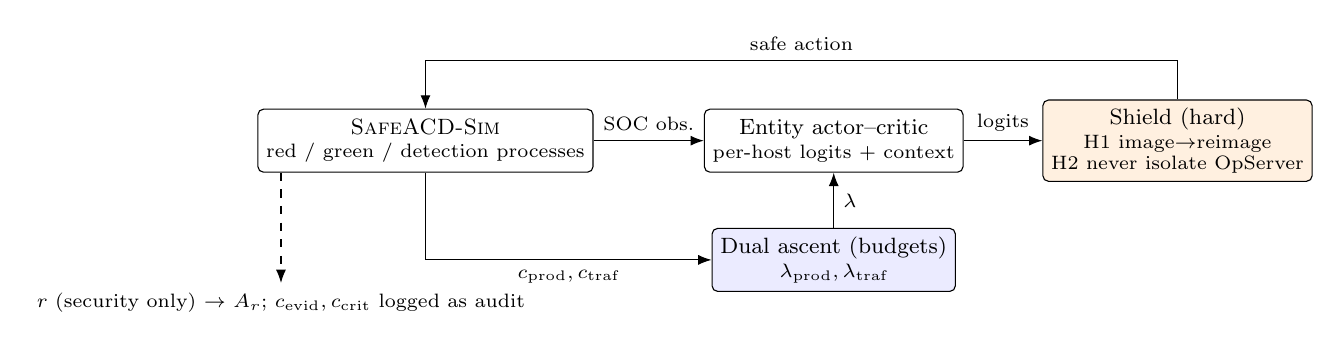
\begin{tikzpicture}[font=\footnotesize, >=Latex,
  box/.style={draw, rounded corners=2pt, align=center, minimum height=8mm, inner sep=3pt},
  hard/.style={box, fill=orange!12}, soft/.style={box, fill=blue!8}]
\node[box, minimum width=30mm] (sim) {\safeacd{}\\[-1pt]\scriptsize red / green / detection processes};
\node[box, right=14mm of sim, minimum width=26mm] (pol) {Entity actor--critic\\[-1pt]\scriptsize per-host logits + context};
\node[hard, right=10mm of pol, minimum width=24mm] (sh) {Shield (hard)\\[-1pt]\scriptsize H1 image$\to$reimage\\[-2pt]\scriptsize H2 never isolate OpServer};
\node[soft, below=7mm of pol, minimum width=26mm] (lag) {Dual ascent (budgets)\\[-1pt]\scriptsize $\lambda_{\text{prod}},\lambda_{\text{traf}}$};
\draw[->] (sim) -- node[above]{\scriptsize SOC obs.} (pol);
\draw[->] (pol) -- node[above]{\scriptsize logits} (sh);
\draw[->] (sh.north) -- ++(0,5mm) -| node[pos=0.25, above]{\scriptsize safe action} (sim.north);
\draw[->] (sim.south) |- node[pos=0.75, below]{\scriptsize $c_{\text{prod}}, c_{\text{traf}}$} (lag.west);
\draw[->] (lag) -- node[right]{\scriptsize $\lambda$} (pol);
\draw[->, dashed] (sim.south west) ++(3mm,0) -- ++(0,-14mm) node[below, align=center]{\scriptsize $r$ (security only) $\to$ $A_r$;\ $c_{\text{evid}}, c_{\text{crit}}$ logged as audit};
\end{tikzpicture}
\caption{\typed{} agent in the loop. Budget harms are priced by Lagrange
multipliers; hard harms are prevented by a preemptive shield that reads only
SOC-observable state. All four harm channels are logged for every method.}
\label{fig:arch}
\end{figure}

\paragraph{Monitor-relative guarantees.}
The shield reads only what a SOC has---tickets and image timestamps---never
the simulator's ground truth. H2 is therefore enforced exactly, whereas H1
holds \emph{relative to the monitor}: a compromise that begins after an image
and is never detected can still lose artefacts on reimage. We measure this
residual rather than claim zero violations by construction.

% ----------------------------------------------------------------------------
\section{The \safeacd{} Simulation Model}
% ----------------------------------------------------------------------------
\paragraph{Structure.}
\safeacd{} is a discrete-time stochastic simulation (100 steps per episode)
of 12 hosts in three subnets mirroring CAGE-2: five user workstations, three
enterprise servers (Ent0--Ent2) and an operational subnet with the
safety-critical OpServer and three OT hosts. Two zone links (user$\to$enterprise,
enterprise$\to$operational) can be blocked. Each step the blue agent acts,
the red agent acts, benign traffic is sampled, alerts are generated, and
reward and costs are emitted (Table~\ref{tab:params}).

\paragraph{Red agents.}
Red progresses along an attack graph: an exploit within a zone needs a
user-level foothold, crossing a zone needs a privileged one; escalation turns
user into privileged access; a privileged foothold on the OpServer allows a
mission \emph{impact}. \textsf{B-line} heads straight for the OpServer;
\textsf{Meander} escalates everywhere and expands subnet by subnet; the
held-out \textsf{Stealthy} attacker is B-line with 30\% dwell and 60\% lower
detection probability. The initial foothold is a random, undetected user host,
and an attacker left without a usable foothold re-phishes with probability 0.1.

\paragraph{Benign traffic and evidence.}
Fifteen weighted business flows (web, file, authentication, historian, control
loop) are active with fixed probabilities; a flow is served only if both
endpoints are online and the zone link is open. Evidence is
\emph{incident-scoped}: the first compromise of a clean host opens an incident;
a forensic image taken afterwards preserves it until the host is reimaged.

\paragraph{Defender interface.}
77 discrete actions: \textsf{Sleep}; per-host \textsf{Analyse},
\textsf{Forensics} (image), \textsf{Remove} (evicts user-level access only),
\textsf{Restore} (reimage, host offline for two steps), \textsf{Isolate},
\textsf{Reconnect}; and \textsf{Block}/\textsf{Unblock} per zone link. The
87-dimensional observation contains, per host, the SOC ticket severity, the
alert raised this step, isolation and reimaging flags, and whether a valid
image exists, plus link states and time.

\begin{table}[t]
\centering
\caption{Main \safeacd{} parameters (defaults in \texttt{safeacd/env.py}).}
\label{tab:params}
\small
\begin{tabular}{ll}
\toprule
Parameter & Value \\
\midrule
Horizon / restore downtime & 100 steps / 2 steps \\
$P$(exploit), $P$(escalate) & 0.75, 0.80 \\
$P$(detect exploit / escalate / impact) & 0.85 / 0.70 / 1.0 (Stealthy: $\times 0.4$) \\
$P$(false alert per host-step), $P$(re-phish) & 0.01, 0.1 \\
Security reward & $-\sum_h v_h\,(0.5\,[\text{user}]+1\,[\text{priv}])-10\,[\text{impact}]$; $v$ = 0.1 users/OT hosts, 1 servers \\
Downtime weights & users 0.1, servers/OT hosts 1, OpServer 2 \\
Budgets $d$ (prod, traf, evid, crit) & 10, 50, 0, 0 per episode \\
\bottomrule
\end{tabular}
\end{table}

\paragraph{Verification and validation.}
Twenty automated tests verify determinism under seeding, the cost semantics
(image-then-reimage costs no evidence; reimage-without-image costs one; the
critical rule; blocked-link traffic loss) and the shield invariants. For
operational validation we ran four reference policies on the evaluation seeds
(Table~\ref{tab:calib}). The ordering matches expert expectation, and the last
row exposes the paper's motivating problem: the policy with the best
\emph{security} return against B-line is the most harmful one. Pilot runs
also revealed two modelling artefacts that we fixed before the main
experiment and report as V\&V lessons: (i) a fixed initial foothold (the
CAGE-2 convention) let every learner quarantine one workstation forever and
freeze the attacker; (ii) alert-scoped evidence created a dead-lock in which
an attacker acting on a host invalidated every new image.

\begin{table}[t]
\centering
\caption{Operational validation with reference policies (100 CRN episodes
per attacker; per-episode means). R: security return; prod/traf: downtime and
blocked-traffic cost. No reference policy destroyed evidence; the reward
hacker isolates the OpServer in every step (100 critical violations).}
\label{tab:calib}
\small
\begin{tabular}{lrrrrrr}
\toprule
& \multicolumn{3}{c}{B-line} & \multicolumn{3}{c}{Meander}\\
\cmidrule(lr){2-4}\cmidrule(lr){5-7}
Policy & R & prod & traf & R & prod & traf\\
\midrule
No defence & $-1172.7$ & 0.0 & 0.0 & $-1131.0$ & 0.0 & 0.0\\
Random & $-528.8$ & 328.8 & 1019.4 & $-387.1$ & 328.8 & 1019.4\\
SOC playbook (image before reimage) & $-78.8$ & 12.5 & 52.4 & $-13.3$ & 3.2 & 31.0\\
``Isolate OpServer + block'' & $-47.6$ & 200.0 & 1319.2 & $-47.6$ & 200.0 & 1319.2\\
\bottomrule
\end{tabular}
\end{table}

% ----------------------------------------------------------------------------
\section{Experimental Design}
% ----------------------------------------------------------------------------
\paragraph{Conditions.}
All learning conditions share one PPO implementation and hyper-parameters
(8 environments $\times$ 256 steps, 10 epochs, minibatch 256, learning rate
$3\cdot10^{-4}$, $\gamma=0.99$, GAE $\lambda=0.95$, clip 0.2, entropy 0.01)
and one \emph{entity-based} actor--critic \citep{symesthompson2024entity}: a
64-unit encoder shared by all hosts, a permutation-invariant pooled context,
a per-host head producing that host's six action logits, a global head for
\textsf{Sleep}/\textsf{Block}/\textsf{Unblock}, and a critic with one reward
and four cost heads. Lagrange multipliers follow clipped, budget-normalised
projected ascent, $\lambda_k\leftarrow\max\bigl(0,\lambda_k+0.05\,\mathrm{clip}((J_k-d_k)/\max(d_k,1),-1,1)\bigr)$,
which bounds overshoot in both directions \citep{stooke2020pid}. Conditions
differ only in safety handling: \textbf{PPO} (security reward only);
\textbf{Shaped}-$\beta$ (reward minus $\beta(c_{\text{prod}}+c_{\text{traf}}+10c_{\text{evid}}+10c_{\text{crit}})$, $\beta=1$
in the main grid, $\beta\in\{0.1,0.3,3,10\}$ in a sweep); \textbf{Lag} (PPO-Lagrangian
on all four channels with $d=(10,50,0,0)$); \textbf{Shield} (security reward
plus shield); and \textbf{\typed{}} (Lagrangian on the two budgets plus shield).
Invalid-action masking is applied everywhere. The budgets encode ``no more
collateral harm than the incumbent playbook'': the playbook's mean downtime
and traffic cost under the training distribution are 7.9 and 41.7.

\paragraph{Protocol.}
Each condition is trained for $10^6$ steps on a uniform B-line/Meander mixture
with ten independent seeds (seeds 1--10; seed 0 was reserved for pilot runs that fixed the architecture and dual step) and three seeds per $\beta$ in the sweep. Each trained stochastic policy is
evaluated for 100 episodes per attacker, including the held-out Stealthy
attacker. Evaluation episode $i$ uses the same seed for every policy, and the
red, green and detection processes draw from independent random streams, so
comparisons use \emph{common random numbers} \citep{law2015simulation}. For RQ3
we additionally deploy the unshielded policies with the shield attached
(``+S''). We report seed-level means with 95\% percentile-bootstrap CIs and
IQM \citep{agarwal2021precipice,henderson2018matters}; pre-registered
comparisons use Mann--Whitney U tests on seed means and, against the
playbook, Wilcoxon signed-rank tests on CRN-paired episodes, all
Holm-corrected. The full protocol is in the artefact
(\texttt{docs/methodology.md}).

% ----------------------------------------------------------------------------
\section{Results}
% ----------------------------------------------------------------------------
\IfFileExists{tables/main.tex}{\begin{table}[t]
\centering
\caption{Deployment performance under the training attacker distribution (B-line/Meander mixture). Mean over seeds with 95\% bootstrap CI over seeds; 100 common-random-number episodes per attacker. Bottom block (RQ3): unshielded policies deployed with the shield attached.}
\label{tab:main}
\setlength{\tabcolsep}{3pt}
\resizebox{\linewidth}{!}{%
\begin{tabular}{lrrrrrrr}
\toprule
Method & Security return $\uparrow$ & Downtime $\downarrow$ & Blocked traffic $\downarrow$ & Evidence destroyed $\downarrow$ & Critical viol. $\downarrow$ & $P$(no hard viol.) $\uparrow$ & $P$(all satisfied) $\uparrow$\\
 & & (budget 10) & (budget 50) & (budget 0) & (budget 0) & & \\
\midrule
SOC playbook & -46.0 & 7.9 & 41.7 & 0.00 & 0.00 & 1.000 & 0.65\\
PPO (reward only) & -1.5 \scriptsize[-2.0, -1.1] & 494.1 \scriptsize[289.0, 668.1] & 1181.0 \scriptsize[950.4, 1395.2] & 4.30 \scriptsize[2.49, 6.77] & 59.82 \scriptsize[33.82, 83.46] & 0.002 \scriptsize[0.000, 0.006] & 0.00\\
Shaped ($\beta$=1) & -36.1 \scriptsize[-40.0, -32.5] & 4.2 \scriptsize[3.6, 4.9] & 21.5 \scriptsize[18.6, 24.6] & 3.02 \scriptsize[2.69, 3.34] & 0.00 \scriptsize[0.00, 0.01] & 0.057 \scriptsize[0.039, 0.079] & 0.06 \scriptsize[0.04, 0.08]\\
PPO-Lagrangian & -60.5 \scriptsize[-65.5, -56.7] & 8.1 \scriptsize[7.0, 9.1] & 54.4 \scriptsize[45.8, 65.7] & 1.01 \scriptsize[0.48, 1.59] & 0.11 \scriptsize[0.05, 0.19] & 0.492 \scriptsize[0.304, 0.680] & 0.34 \scriptsize[0.22, 0.46]\\
PPO+Shield & -1.6 \scriptsize[-1.8, -1.4] & 196.8 \scriptsize[60.5, 341.3] & 845.6 \scriptsize[661.2, 1056.0] & 0.01 \scriptsize[0.00, 0.02] & 0.00 & 0.990 \scriptsize[0.982, 0.998] & 0.00\\
Typed (Lag+Shield) & -61.0 \scriptsize[-67.7, -55.1] & 8.0 \scriptsize[7.0, 9.1] & 42.5 \scriptsize[35.4, 49.7] & 0.03 \scriptsize[0.01, 0.04] & 0.00 & 0.977 \scriptsize[0.962, 0.988] & 0.69 \scriptsize[0.64, 0.74]\\
\midrule
PPO, shield at deploy & -101.6 \scriptsize[-194.0, -46.2] & 312.6 \scriptsize[167.3, 450.5] & 1021.3 \scriptsize[788.9, 1238.5] & 0.01 \scriptsize[0.00, 0.01] & 0.00 & 0.994 \scriptsize[0.987, 0.999] & 0.00 \scriptsize[0.00, 0.00]\\
Shaped, shield at deploy & -427.3 \scriptsize[-519.0, -318.1] & 9.7 \scriptsize[6.3, 13.4] & 73.4 \scriptsize[46.8, 105.7] & 0.04 \scriptsize[0.01, 0.07] & 0.00 & 0.966 \scriptsize[0.937, 0.992] & 0.52 \scriptsize[0.38, 0.65]\\
PPO-Lag, shield at deploy & -131.8 \scriptsize[-195.0, -76.4] & 8.5 \scriptsize[6.8, 10.0] & 89.9 \scriptsize[59.4, 124.5] & 0.02 \scriptsize[0.01, 0.05] & 0.00 & 0.981 \scriptsize[0.966, 0.993] & 0.49 \scriptsize[0.35, 0.59]\\
\bottomrule
\end{tabular}}
\end{table}
}{\todo{run scripts/analyze.py}}

\begin{figure}[t]
\centering
\IfFileExists{figures/pareto.pdf}{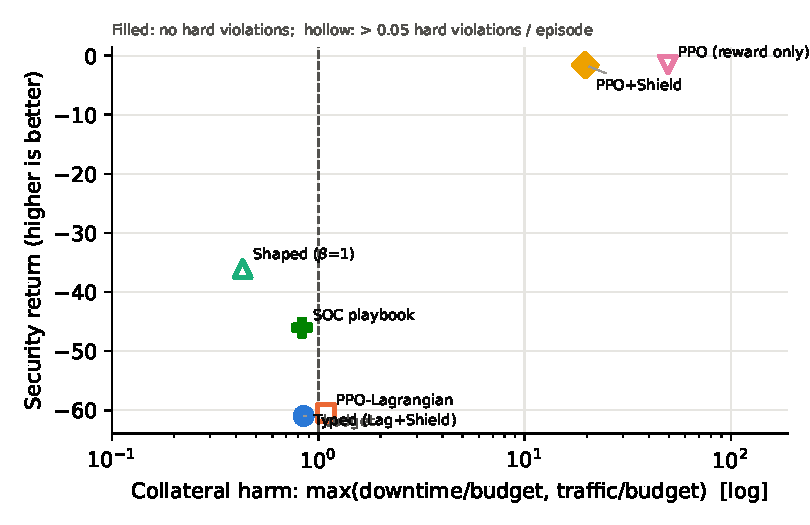
\includegraphics[width=0.62\linewidth]{figures/pareto.pdf}}{\todo{pareto figure}}
\caption{Security return versus normalised collateral harm (log scale) under
the training distribution; hollow markers indicate hard-constraint violations.}
\label{fig:pareto}
\end{figure}

\begin{figure}[t]
\centering
\IfFileExists{figures/learning.pdf}{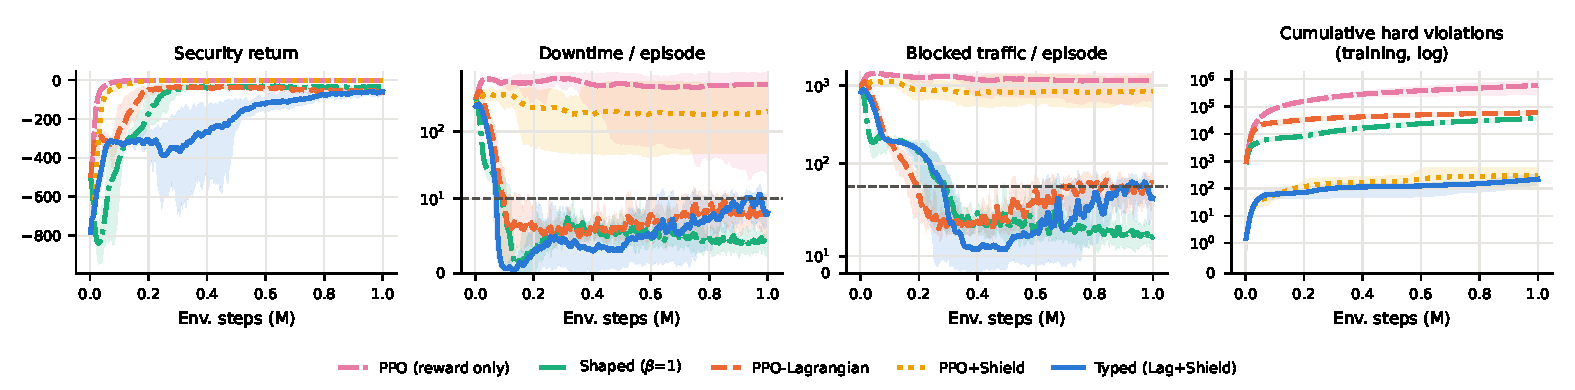
\includegraphics[width=\linewidth]{figures/learning.pdf}}{\todo{learning curves}}
\caption{Training dynamics (mean and 10--90\% band over seeds). Dashed lines
are budgets. The right panel counts hard violations committed \emph{during
training} (log scale).}
\label{fig:learning}
\end{figure}

\paragraph{RQ1: Maximising reward is maximally harmful, and penalties are a price.}
Reward-only PPO reaches a near-perfect security return
(\resTrainPpoR; Table~\ref{tab:main}) by severing the OT controller for
\resTrainPpoCrit{} of 100 steps per episode, keeping production hosts offline
for \resTrainPpoProd{} host-steps (budget 10), blocking \resTrainPpoTraf{}
units of legitimate traffic (budget 50) and destroying evidence
\resTrainPpoEvid{} times per episode. The shield alone (PPO+Shield) removes
the hard violations but not the budget harm (\resTrainShieldProd{} and
\resTrainShieldTraf). Reward shaping with $\beta=1$ keeps both budgets and
almost never isolates the controller, yet destroys evidence
\resTrainShapedEvid{} times per episode and violates a hard constraint in
\resTrainShapedHardFreePctViol\% of episodes, although each destruction costs
ten times a server-step of downtime. The agent has simply priced the
irreversible harm in, and that is where its higher security return
(\resTrainShapedR{} vs.\ \resTrainTypedR{} for \typed;
$p_{\text{Holm}}=\pTypedVsShapedReturn$) comes from. The $\beta$ sweep
(Figure~\ref{fig:shaping}) shows the trade-off:
\begin{itemize}
\item with $\beta\le 1$, evidence is destroyed in at least
\resTrainShapedHardFreePctViol\% of episodes ($\beta=0.3$:
\resTrainShapedThreeTenthsHardFreePctViol\%);
\item with $\beta\ge 3$, harm disappears but security collapses to
\resTrainShapedThreeR{} ($\beta=3$) and \resTrainShapedTenR{} ($\beta=10$).
\end{itemize}
No penalty weight gives both safety and security, so the weight is a tuning
burden, not a guarantee.

\paragraph{RQ2: Typing the constraints.}
\typed{} satisfies both budgets in expectation (downtime \resTrainTypedProd,
traffic \resTrainTypedTraf). It is free of hard violations in
\resTrainTypedHardFreePct\% of episodes (\nhardTrainTyped{} episodes with a
violation), all of them monitor-relative H1 misses; the OT rule is never
violated. PPO-Lagrangian treats evidence and the OT rule as zero-budget
constraints. It ends training with multipliers of
$\lambda_{\text{evid}}\approx\lamFinalLagEvidence$ and
$\lambda_{\text{crit}}\approx\lamFinalLagCritical$, yet still commits a hard
violation in \resTrainLagHardFreePctViol\% of episodes
($p_{\text{Holm}}=\pTypedVsLagHardFree$) and exceeds the traffic budget on
average (\resTrainLagTraf). Expectation constraints are the wrong contract
for irreversible harm: a multiplier only grows \emph{after} violations have
happened, so violations accumulate throughout training
(Figure~\ref{fig:learning}, right) and persist at deployment. Security is
indistinguishable (\resTrainTypedR{} vs.\ \resTrainLagR;
$p_{\text{Holm}}=\pTypedVsLagReturn$), and \typed{} meets all four
constraints in about twice as many episodes (\resTrainTypedSatPct\% vs.\
\resTrainLagSatPct\%; $p_{\text{Holm}}=\pTypedVsLagSatAll$). Against the
incumbent playbook, whose mean harm defines the budgets, \typed{} incurs the
same downtime and traffic (paired CRN tests,
$p_{\text{Holm}}=\pTypedVsPlaybookCostProd$ and
$\pTypedVsPlaybookCostTraffic$) but a lower security return
(\resTrainTypedR{} vs.\ \resTrainPlaybookR;
$p_{\text{Holm}}=\pTypedVsPlaybookReturn$).

\paragraph{RQ3: The shield belongs in the training loop.}
Attaching the shield only at deployment (bottom block of
Table~\ref{tab:main}) removes most hard violations, but the policy then acts
in states its training never visited.
\begin{itemize}
\item \textbf{Shaped PPO} learned ``reimage without imaging'' as its main
remediation, and its security collapses (\resTrainShapedR{} $\to$
\resTrainShapedDeployR; $p_{\text{Holm}}=\pShapedVsShapedDeployReturn$).
\item \textbf{PPO-Lagrangian} degrades on average (\resTrainLagR{} $\to$
\resTrainLagDeployR; IQM \resTrainLagRIqm{} $\to$ \resTrainLagDeployRIqm)
and its traffic rises to \resTrainLagDeployTraf. The effect varies widely
across seeds and is not significant after correction
($p_{\text{Holm}}=\pLagVsLagDeployReturn$).
\item \textbf{Reward-only PPO} with the shield still exceeds the budgets by
an order of magnitude.
\end{itemize}
Training with the shield lets the policy learn the ``image, then reimage''
sequence. \typed{} reaches a better return than every deploy-only variant at
equal or lower harm.

\paragraph{RQ4: A held-out attacker.}
Against the unseen low-and-slow attacker (Table~\ref{tab:ood}) every defender
degrades, and every one, including the playbook, exceeds the budgets: budgets
hold only in expectation under the training distribution. H2 still holds by
construction. H1's monitor-relative gap widens as detection gets worse:
\typed{} is free of hard violations in \resOodTypedHardFreePct\% of episodes,
against \resOodLagHardFreePct\% for PPO-Lagrangian and
\resOodShapedHardFreePct\% for shaping. The residuals come from images that
predate a new, undetected compromise. Adding an image-freshness window to H1
at deployment (Table~\ref{tab:freshness}) narrows that window. Requiring the
image to be at most three steps old raises the violation-free rate against
the stealthy attacker from \freshOodKNoneHardFreePct\% to
\freshOodKThreeHardFreePct\% (one step: \freshOodKOneHardFreePct\%), at a
small cost in security. Under the training distribution, however, tightening
the rule only at deployment costs security (\freshTrainKNoneR{} $\to$
\freshTrainKOneR{} for one step) and pushes traffic towards or over budget
(\freshTrainKOneTraf). This is the same train/deploy mismatch as in RQ3, and
it argues for training with the rule that will be deployed.

\IfFileExists{tables/ood.tex}{\begin{table}[t]
\centering
\caption{Out-of-distribution evaluation against the held-out low-and-slow (Stealthy) attacker.}
\label{tab:ood}
\setlength{\tabcolsep}{3pt}
\resizebox{\linewidth}{!}{%
\begin{tabular}{lrrrrrrr}
\toprule
Method & Security return $\uparrow$ & Downtime $\downarrow$ & Blocked traffic $\downarrow$ & Evidence destroyed $\downarrow$ & Critical viol. $\downarrow$ & $P$(no hard viol.) $\uparrow$ & $P$(all satisfied) $\uparrow$\\
 & & (budget 10) & (budget 50) & (budget 0) & (budget 0) & & \\
\midrule
SOC playbook & -194.8 & 32.7 & 133.0 & 0.00 & 0.00 & 1.000 & 0.03\\
PPO (reward only) & -10.5 \scriptsize[-18.8, -4.2] & 502.0 \scriptsize[294.5, 677.2] & 1194.3 \scriptsize[963.5, 1411.3] & 5.31 \scriptsize[2.13, 9.79] & 60.77 \scriptsize[34.42, 84.86] & 0.002 \scriptsize[0.000, 0.006] & 0.00\\
Shaped ($\beta$=1) & -218.1 \scriptsize[-246.2, -194.8] & 31.8 \scriptsize[26.6, 36.6] & 128.6 \scriptsize[108.2, 147.2] & 6.86 \scriptsize[5.52, 7.97] & 0.03 \scriptsize[0.01, 0.06] & 0.009 \scriptsize[0.000, 0.026] & 0.00\\
PPO-Lagrangian & -273.7 \scriptsize[-294.2, -250.2] & 37.7 \scriptsize[34.6, 40.5] & 177.7 \scriptsize[162.3, 192.5] & 2.47 \scriptsize[0.86, 4.32] & 0.76 \scriptsize[0.21, 1.38] & 0.334 \scriptsize[0.158, 0.533] & 0.01 \scriptsize[0.00, 0.01]\\
PPO+Shield & -4.5 \scriptsize[-7.3, -2.7] & 200.3 \scriptsize[62.1, 347.7] & 852.1 \scriptsize[663.5, 1066.8] & 0.01 \scriptsize[0.00, 0.02] & 0.00 & 0.993 \scriptsize[0.984, 1.000] & 0.00\\
Typed (Lag+Shield) & -226.4 \scriptsize[-249.9, -200.3] & 32.1 \scriptsize[27.5, 36.1] & 132.8 \scriptsize[112.8, 149.9] & 0.11 \scriptsize[0.06, 0.16] & 0.00 & 0.901 \scriptsize[0.853, 0.948] & 0.06 \scriptsize[0.01, 0.14]\\
\bottomrule
\end{tabular}}
\end{table}
}{}
\IfFileExists{tables/freshness.tex}{\begin{table}[t]\centering
\caption{Typed policies deployed with H1 tightened by an image-freshness window (evaluation only; mean over seeds, 100 CRN episodes per attacker).}
\label{tab:freshness}\small
\begin{tabular}{llrrrr}\toprule
Attackers & H1 variant & Return & Traffic & Evidence destroyed & $P$(no hard viol.)\\\midrule
training & H1 (no window) & -61.0 & 42.5 & 0.025 & 0.977\\
training & H1 + image age $\le$ 3 & -79.9 & 48.1 & 0.013 & 0.988\\
training & H1 + image age $\le$ 1 & -104.1 & 55.7 & 0.003 & 0.997\\
stealthy (OOD) & H1 (no window) & -226.4 & 132.8 & 0.108 & 0.901\\
stealthy (OOD) & H1 + image age $\le$ 3 & -231.2 & 131.6 & 0.021 & 0.980\\
stealthy (OOD) & H1 + image age $\le$ 1 & -241.3 & 128.1 & 0.005 & 0.996\\
\bottomrule\end{tabular}\end{table}
}{}

\begin{figure}[t]
\centering
\IfFileExists{figures/shaping.pdf}{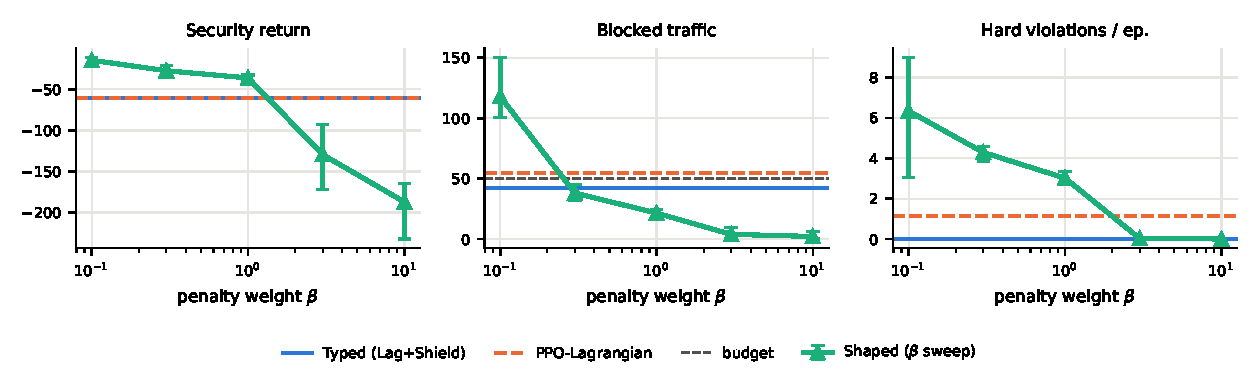
\includegraphics[width=0.9\linewidth]{figures/shaping.pdf}}{\todo{shaping sweep}}
\caption{Reward shaping across penalty weights $\beta$ (mean and 95\% CI over
seeds), with \typed{} and PPO-Lagrangian as horizontal references.}
\label{fig:shaping}
\end{figure}

% ----------------------------------------------------------------------------
\section{Discussion and Threats to Validity}
% ----------------------------------------------------------------------------
\paragraph{Implications for ACD design.}
Three lessons carry over to other environments.
(i)~\emph{Separate the signals.} With harm emitted as cost channels rather
than folded into reward, any method's collateral damage is measurable,
including a reward-only baseline that looks best on the usual security
metric.
(ii)~\emph{Choose the mechanism by type.} A penalty or a multiplier turns an
irreversible harm into a price. A shield that encodes the operational rule
the SOC already follows (image before reimage; never sever the OT
controller) prevents it, and leaves budget-type harms to the Lagrangian
relaxation, which handles them well.
(iii)~\emph{State guarantees relative to the monitor.} A shield built on SOC
observables is only as good as detection. Reporting residuals, and testing
against a stealthier attacker, makes this limit visible rather than hiding it
behind ``safe by construction''.
In this small network a well-engineered playbook remains a strong baseline,
with better security at the same harm. The contribution here is not that RL
beats playbooks, but how a learned defender must be constrained before it
can be trusted alongside one.

\paragraph{Threats.}
\emph{Internal:} hyper-parameters were shared, not tuned per condition; the
$\beta$ sweep bounds the effect of tuning the shaping baseline.
\emph{Construct:} downtime and traffic are proxies, and evidence is modelled
as a binary per-incident property, whereas real artefacts are graded by
volatility \citep{rfc3227}. \emph{External:} one 12-host topology with
scripted attackers; our claims concern safety \emph{mechanisms}, not
deployment-ready agents; porting the cost channels to CybORG/CAGE-4 is future
work. \emph{Conclusion:} ten seeds, CRN pairing, bootstrap CIs and Holm
correction; near-zero violation rates are reported with exact binomial upper
bounds.

% ----------------------------------------------------------------------------
\section{Conclusion}
% ----------------------------------------------------------------------------
A cyber-defence agent should not be allowed to buy security with harm it
cannot undo. In \safeacd{}, reward maximisation bought security by severing
the OT controller and destroying evidence. Penalties and Lagrange multipliers
turned that harm into a price the agent was willing to pay. A typed design,
with budgets for recoverable harm and an observation-based shield for
irreversible harm, kept collateral damage within the playbook's envelope and
made hard violations rare and attributable to monitoring gaps. Next steps
are to port the cost channels to CybORG CAGE-4, model graded (volatility-ordered)
evidence, and synthesise shields from SOC runbooks.

\paragraph{Artefact availability.} Simulator, agents, configuration, raw
evaluation records and analysis scripts: \todo{anonymised repository / Zenodo DOI}.

\bibliographystyle{plainnat}
\bibliography{refs}
\end{document}
